\documentclass[12pt, a4paper]{article}
\usepackage[text={6.5in,9.6in}]{geometry}
\usepackage[utf8]{inputenc}
\usepackage{graphicx}
\usepackage{geometry}
\usepackage{float}
\usepackage{amsmath}
\usepackage{slashed}
\usepackage{multicol}
\usepackage{hyperref}
\usepackage[T1]{fontenc}
\usepackage{upgreek}
\usepackage{textgreek}
\usepackage{helvet}
\usepackage{hepparticles}
\usepackage{heppennames}
\usepackage{caption}
\usepackage{subcaption}
\usepackage{cite}
\usepackage{amsmath,amssymb,braket,tikz}
\usetikzlibrary{tikzmark,calc}
\usetikzlibrary{positioning}
%\renewcommand{\baselinestretch}{1.5}
%\usepackage{ptdr-definitions}
%\usepackage{}

%\usepackage{utopia}
\hypersetup{
	colorlinks=true,
	citecolor=red,
	linkcolor=blue,
	filecolor=magenta,      
	urlcolor=cyan,
	%pdftitle={Overleaf Example},
	pdfpagemode=FullScreen,
}
\title{\textbf{Search for Higgs boson and top squark in di-$\uptau$ final state with the CMS detector}}
\author{\textbf{Saikat Karmakar}\\
Department of High Energy Physics, TIFR, Mumbai\\
\\
Ph.D. Supervisors:\\
Prof. Sudeshna Banerjee, DHEP, TIFR, Mumbai \\
(Supervisor till January 2019, afterwards co-supervisor)\\
Prof. Monoranjan Guchait, DHEP, TIFR, Mumbai\\
 (Supervisor since February 2019)\\
 \\
Registration no: PHYS-383}

\date{}
\newcommand{\pt}{\ensuremath{p_{\mathrm{T}}}\xspace}
\newcommand{\ptmiss}{\ensuremath{\pt^\text{miss}}}
\newcommand{\mT}{\ensuremath{m_{\mathrm{T}}}\xspace}
\newcommand{\ptvec}{\ensuremath{{\vec p}_{\mathrm{T}}}\xspace}
\newcommand{\ptvecmiss}{\ensuremath{{\vec p}_{\mathrm{T}}^{\kern1pt\text{miss}}}\xspace}
\newcommand{\mTii}{\ensuremath{m_{\mathrm{T2}}}\xspace}
\newcommand{\ST}{\ensuremath{S_{\mathrm{T}}}\xspace}
\newcommand{\ET}{\ensuremath{E_{\mathrm{T}}}\xspace}
\newcommand{\mf}{\ensuremath{m_{\mathrm{f}}}}
\newcommand{\yt}{\ensuremath{y_{\mathrm{t}}}}
\newcommand{\yf}{\ensuremath{y_{\mathrm{f}}}}
\newcommand{\DR}{\Delta\text{R}}
\newcommand{\GeV}{\ensuremath{\text{Ge\hspace{-.08em}V}}{}\xspace}
%\DeclareRobustCommand{\PZGc}{{\HepParticle{\PZ}{\upchi}{}}\Xspace}
\DeclareRobustCommand{\PW}{{\HepParticle{W}{}{}}\xspace}
\DeclareRobustCommand{\PH}{{\HepParticle{H}{}{}}\xspace}
\DeclareRobustCommand{\PZ}{{\HepParticle{Z}{}{}}\xspace}
\DeclareRobustCommand{\PQq}{\HepParticle{q}{}{}} % quark (generic)
\DeclareRobustCommand{\PQd}{{\HepParticle{d}{}{}}\xspace} % down quark
\DeclareRobustCommand{\PQu}{{\HepParticle{u}{}{}}\xspace} % up quark
\DeclareRobustCommand{\PQs}{{\HepParticle{s}{}{}}\xspace} % strange quark
\DeclareRobustCommand{\PQc}{{\HepParticle{c}{}{}}\xspace} % charm quark
\DeclareRobustCommand{\PQb}{{\HepParticle{b}{}{}}\xspace} % bottom quark
\DeclareRobustCommand{\PQt}{\HepParticle{t}{}{}} % top quark
\DeclareRobustCommand{\PQbpr}{{\HepParticle{\PQb}{}{\prime}}\xspace} % bottom prime quark
\DeclareRobustCommand{\PQtpr}{{\HepParticle{\PQt}{}{\prime}}\xspace} % top prime quark

\DeclareRobustCommand{\PAQq}{{\HepAntiParticle{\PQq}{}{}}\xspace} % anti-quark (generic)
\DeclareRobustCommand{\PAQd}{{\HepAntiParticle{\PQd}{}{}}\xspace} % down anti-quark
\DeclareRobustCommand{\PAQu}{{\HepAntiParticle{\PQu}{}{}}\xspace} % up anti-quark
\DeclareRobustCommand{\PAQs}{{\HepAntiParticle{\PQs}{}{}}\xspace} % strange anti-quark
\DeclareRobustCommand{\PAQc}{{\HepAntiParticle{\PQc}{}{}}\xspace} % charm anti-quark
\DeclareRobustCommand{\PAQb}{{\HepAntiParticle{\PQb}{}{}}\xspace} % bottom anti-quark
\DeclareRobustCommand{\PAQt}{{\HepAntiParticle{\PQt}{}{}}\xspace} % top anti-quark
\DeclareRobustCommand{\PAQbpr}{{\HepAntiParticle{\PQb}{}{\prime}}\xspace} % bottom prime anti-quark
\DeclareRobustCommand{\PAQtpr}{{\HepAntiParticle{\PQt}{}{\prime}}\xspace} % top prime anti-quark

\DeclareRobustCommand{\Pe}{{\HepParticle{e}{}{}}\xspace} % electron
\DeclareRobustCommand{\Pepm}{{\HepParticle{\Pe}{}{\pm}}\xspace} % e plus/minus
\DeclareRobustCommand{\Pemp}{{\HepParticle{\Pe}{}{\mp}}\xspace} % e minus/plus
\DeclareRobustCommand{\Pem}{{\HepParticle{\Pe}{}{-}}\xspace} % electron
\DeclareRobustCommand{\Pep}{{\HepParticle{\Pe}{}{+}}\xspace} % positron

\DeclareRobustCommand{\PGm}{{\HepParticle{\upmu}{}{}}\xspace} % muon
\DeclareRobustCommand{\PGmpm}{{\HepParticle{\PGm}{}{\pm}}\xspace} % mu plus/minus
\DeclareRobustCommand{\PGmm}{{\HepParticle{\PGm}{}{-}}\xspace} % muon
\DeclareRobustCommand{\PGmp}{{\HepParticle{\PGm}{}{+}}\xspace} % anti-muon

\DeclareRobustCommand{\PGt}{{\HepParticle{\uptau}{}{}}\xspace} % tau
\DeclareRobustCommand{\PGtpm}{{\HepParticle{\PGt}{}{\pm}}\xspace} % tau plus/minus
\DeclareRobustCommand{\PGtm}{{\HepParticle{\PGt}{}{-}}\xspace} % tau lepton
\DeclareRobustCommand{\PGtp}{{\HepParticle{\PGt}{}{+}}\xspace} % anti-tau
\DeclareRobustCommand{\PAGt}{\HepAntiParticle{\PGt}{}{}\xspace} % generic anti-tau

\DeclareRobustCommand{\PGn}{{\HepParticle{\upnu}{}{}}\xspace} % neutrino
\DeclareRobustCommand{\PGne}{{\HepParticle{\PGn}{\!\Pe}{}}\xspace} % electron neutrino
\DeclareRobustCommand{\PGnGm}{{\HepParticle{\PGn}{\!\PGm}{}}\xspace} % muon neutrino
\DeclareRobustCommand{\PGnGt}{{\HepParticle{\PGn}{\!\PGt}{}}\xspace} % tau neutrino

\DeclareRobustCommand{\PSQt}{{\HepSusyParticle{\PQt}{}{}}\xspace} % top squark (stop)
\DeclareRobustCommand{\PSQtL}{{\HepSusyParticle{\PQt}{L}{}}\xspace}
\DeclareRobustCommand{\PSQtR}{{\HepSusyParticle{\PQt}{R}{}}\xspace}
\DeclareRobustCommand{\PSQtDo}{{\HepSusyParticle{\PQt}{1}{}}\xspace}
\DeclareRobustCommand{\PSQtDt}{{\HepSusyParticle{\PQt}{2}{}}\xspace}
\DeclareRobustCommand{\PASQt}{{\HepSusyAntiParticle{\PQt}{}{}}\xspace} % anti-top squark (stop)
\DeclareRobustCommand{\PASQtL}{{\HepSusyAntiParticle{\PQt}{L}{}}\xspace}
\DeclareRobustCommand{\PASQtR}{{\HepSusyAntiParticle{\PQt}{R}{}}\xspace}
\DeclareRobustCommand{\PASQtDo}{{\HepSusyAntiParticle{\PQt}{1}{}}\xspace}
\DeclareRobustCommand{\PASQtDt}{{\HepSusyAntiParticle{\PQt}{2}{}}\xspace}

\DeclareRobustCommand{\PSGt}{{\HepSusyParticle{\PGt}{}{}}\xspace} % stau
\DeclareRobustCommand{\PSGtmDo}{{\HepSusyParticle{\PGt}{1}{-}}\xspace} % stau
\DeclareRobustCommand{\PSGtmDt}{{\HepSusyParticle{\PGt}{2}{-}}\xspace} % stau
\DeclareRobustCommand{\PSGtpDo}{{\HepSusyParticle{\PGt}{1}{+}}\xspace} % stau
\DeclareRobustCommand{\PSGtpDt}{{\HepSusyParticle{\PGt}{2}{+}}\xspace} % stau
\DeclareRobustCommand{\PSGtL}{{\HepSusyParticle{\PGt}{L}{}}\xspace} % stau
\DeclareRobustCommand{\PSGtR}{{\HepSusyParticle{\PGt}{R}{}}\xspace} % stau
\DeclareRobustCommand{\PSGtDo}{{\HepSusyParticle{\PGt}{1}{}}\xspace} % stau
\DeclareRobustCommand{\PSGtDt}{{\HepSusyParticle{\PGt}{2}{}}\xspace} % stau
\DeclareRobustCommand{\PSGnGt}{{\HepSusyParticle{\PGn}{{\PGt}}{}}\xspace} % tau sneutrino
\DeclareRobustCommand{\PSGnGtDo}{{\HepSusyParticle{\PGn}{{\PGt}1}{}}\xspace}
\DeclareRobustCommand{\PSGnGtDt}{{\HepSusyParticle{\PGn}{{\PGt}2}{}}\xspace}

\DeclareRobustCommand{\PSGc}{{\HepSusyParticle{\upchi}{}{}}\xspace} % chargino/neutralino
\DeclareRobustCommand{\PSGcz}{{\HepParticle{\PSGc}{}{0}}\xspace} % neutralino
\DeclareRobustCommand{\PSGczDo}{{\HepParticle{\PSGc}{1}{0}}\xspace}
\DeclareRobustCommand{\PSGczDt}{{\HepParticle{\PSGc}{2}{0}}\xspace}
\DeclareRobustCommand{\PSGczDT}{{\HepParticle{\PSGc}{3}{0}}\xspace}
\DeclareRobustCommand{\PSGczDf}{{\HepParticle{\PSGc}{4}{0}}\xspace}
\DeclareRobustCommand{\PSGcm}{{\HepParticle{\PSGc}{}{-}}\xspace} % chargino -
\DeclareRobustCommand{\PSGcp}{{\HepParticle{\PSGc}{}{+}}\xspace} % chargino +
\DeclareRobustCommand{\PSGcpm}{{\HepParticle{\PSGc}{}{\pm}}\xspace} % chargino
\DeclareRobustCommand{\PSGcmDo}{{\HepParticle{\PSGc}{1}{-}}\xspace}
\DeclareRobustCommand{\PSGcpDo}{{\HepParticle{\PSGc}{1}{+}}\xspace}
\DeclareRobustCommand{\PSGcpmDo}{{\HepParticle{\PSGc}{1}{\pm}}\xspace}
\DeclareRobustCommand{\PSGcmDt}{{\HepParticle{\PSGc}{2}{-}}\xspace}
\DeclareRobustCommand{\PSGcpDt}{{\HepParticle{\PSGc}{2}{+}}\xspace}
\DeclareRobustCommand{\PSGcpmDt}{{\HepParticle{\PSGc}{2}{\pm}}\xspace}
\DeclareRobustCommand{\PSWpm}{{\HepSusyParticle{\PW}{}{\pm}}\xspace}
\DeclareRobustCommand{\PSWz}{{\HepSusyParticle{\PW}{}{0}}\xspace}
\DeclareRobustCommand{\PSBz}{{\HepSusyParticle{B}{}{0}}\xspace}
\DeclareRobustCommand{\PSH}{{\HepSusyParticle{\PH}{}{}}\xspace}

\newcommand{\ttbar}{\PQt{}\PAQt} % t-tbar
\newcommand{\mh}{\ensuremath{m_{h}}}
\newcommand{\tauh}{\ensuremath{\PGt_\mathrm{h}}\xspace}
\newcommand{\ttH}{\ttbar\PH}
\newcommand{\CLs}{\ensuremath{\text{CL}_\text{s}}\xspace}
\newcommand{\CL}{\ensuremath{\text{CL}}\xspace}

%\input{ptdr-def.tex}
\begin{document}

\begin{titlepage}
\maketitle
\thispagestyle{empty}
\end{titlepage}

\begin{itemize}
{\huge
\item[\textbf{1}]\textbf{ Publications relevant to the thesis}}
	\begin{itemize}
		\item[1.]\textit{Title:} ~~\textbf{Measurement of the Higgs boson production rate in association with top quarks in final states with electrons, muons, and hadronically decaying tau leptons at $\sqrt{s}=13$ TeV}
		\item[] \textit{Status:} \textbf{Published in EPJC (hep-ex 2011.03652v2) on behalf of the CMS collaboration}
		\item[]\textit{DOI:}~~~ \href{https://link.springer.com/article/10.1140/epjc/s10052-021-09014-x}{	10.1140/epjc/s10052-021-09014-x} 
%	\end{itemize}

%\vspace{0.25cm}
%{\huge
%	\item[\textbf{2}]\textbf{ Under review}}
%	\begin{itemize}
		\item[2.] \textit{Title:}~~ \textbf{Search for top squark pair production in a final
			state with two tau leptons in proton-proton collisions at $\sqrt{s} = 13$ TeV}
		\item[]\textit{Status:} \textbf{Under collaboration review. Target journal JHEP on behalf of CMS collaboration. [Pre-approval talk is given and it is preapproved.]}
	\end{itemize}

\vspace{0.5cm}
{\huge
	\item[\textbf{2}]\textbf{ Other publications}}\\
		\begin{itemize}
		\item[1.]\textit{Title:}~~ \textbf{Performance of missing transverse momentum reconstruction in events containing a photon and jets collected by CMS during proton-proton collisions at $\sqrt{s} = 13$ TeV in 2018}
		\item[]\textit{Status:}~~~\textbf{CMS Detector Performance Summary (DPS) note released.}
		\item[]\textit{DPS note:} \href{https://cds.cern.ch/record/2723010/files/DP2020_031.pdf}{CMS DP-2020/031}
	\end{itemize}

\vspace{0.5cm}
{\huge
	\item[\textbf{3}]\textbf{ CMS internal documents}}\\
	\begin{itemize}
	\item[1.]\textit{Title:}~~~\textbf{Measurement of the Higgs boson production in association
		with top quarks in final states with electrons, muons and hadronic taus using the full Run 2 dataset}
	\item[]\textit{CMS internal note:}~~~\textbf{CMS AN-19-111} [Related to publication 1]
	\item[]\textit{Co-authors:} Sudeshna Banerjee, Christian Veelken et al.
	
	\item[2.]\textit{Title:}~~~\textbf{Search for top squark pair production in a di-$\tau$ final state in semileptonic mode at $\sqrt{s} = 13$ TeV with the CMS detector with the full Run 2 dataset}
	\item[]\textit{CMS internal note:}~~~\textbf{CMS AN-20-123} [Related to analysis 2]
	\item[]\textit{Co-authors:} Sudeshna Banerjee, Soham Bhatacharya, Monoranjan Guchait, Gobinda
	Majumder, Seema Sharma
	
	\item[3.]\textit{Title:}~~~\textbf{Performance of missing transverse momentum in pp collision at 13 TeV with the full Run2 dataset}
	\item[]\textit{CMS internal note:}~~~\textbf{CMS AN-21-167} [Related to public document 3]
	\item[]\textit{Co-authors:} Pallabi Das, Saranya Ghosh
	\end{itemize}
\end{itemize}
\thispagestyle{empty}
\clearpage


\tableofcontents
\thispagestyle{empty}
\clearpage
\setcounter{page}{1}
\section{Introduction}\label{intro}
The Compact Muon Solenoid (CMS) experiment\cite{CMS:2008xjf} at the Large Hadron Collider (LHC) has successfully collected high quality data from proton-proton collision during Run 2 (2016-2018) phase. After the discovery of Higgs boson (\PH) by the CMS and ATLAS experiments in 2012  \cite{CMS:2012qbp,ATLAS:2012yve}, now it is time to measure all of it's properties to prove that it is indeed the standard model (SM) Higgs. Despite the tremendous success of the SM, several important problems such as the presence of dark matter, stabilization of Higgs mass etc. indicate that the SM is not the complete description of nature. It motivates to look for physics beyond the SM (BSM).
\begin{itemize} 
\item In the SM, the Yukawa coupling $\yf$ of the \PH boson to the fermions is proportional to the fermion mass $\mf$  and is given by $\yf=\sqrt{2}\mf/v$, where $v\approx 246$ \GeV is the vacuum expectation value of the Higgs field. With a mass $m_{\text{t}}=173.34\pm 0.76$ \GeV\cite{ATLAS:2014wva}, the top quark is the heaviest fermion known till date, and its Yukawa coupling $\yt$ is of the order one. The large mass of the top quark indicate that it plays a special role in the mechanism of electroweak symmetry breaking\cite{Dobrescu:1997nm,Chivukula:1998wd,Delepine:1995qs}. Deviation of $\yt$ from the SM prediction would unambiguously indicate the presence of new physics beyond the SM, and thus the determination of $\yt$ is of special interest in the study of the Higgs boson. We have carried out a search for associated production of Higgs boson with a pair of top and anti-top quark in one lepton (electron or muon) and one hadronically decaying $\PGt$ final state whose details and results are presented in Section \ref{ttH}.

\item Till now all the properties of the Higgs boson discovered at the LHC follows the SM predictions. However, SM can not explain the large corrections to the Higgs mass due to the top quark loops. Supersymmetry (SUSY), which predicts a bosonic (fermionic) partner of each SM fermion (boson) can provide a solution of the \PH mass stability by introducing a superpartner of the top quark, namely the top squark ($\PSQt$). Moreover, the superpartners of SM Higgs (higgsinos) and the gauge bosons (gauginos) mix to give neutralinos and charginos. Interestingly the lightest neutralino can be a possible dark matter candidate in the R-parity conserving SUSY scenarios\cite{FARRAR1978575}. %These are some of the reasons that SUSY is one of the most widely studied Beyond Standard Model (BSM) theories. 
Several SUSY searches in multi-lepton and multi-jet final states are carried out by both CMS and ATLAS experiment to look for SUSY particles gluinos, squarks and electroweak gauginos. The leptons (\Pe/\PGm) and jets originate primarily EW gaugino decays in the SUSY cascade chain. But these final states are not sensitive for the SUSY scenario when $\tan\beta=v_{u}/v_{d}$ is high, or the chargino and neutralino becomes higgsino like. Here $v_{u}$ and $v_{d}$ are the vacuum expectation values corresponding to the two Higgs doublet predicted by the Minimal Supersymmetric Standard Model (MSSM). For high $\tan\beta$/ higgsino like scenario, the third generation slepton-lepton couplings are enhanced, leading to a final state with tau lepton. In order to probe such a scenario top squark pair production search is carried out with tau leptons in the final state. In this search we consider the one tau lepton decays leptonically and other tau lepton decays hadronically, whose details and results are presented in Section \ref{stop_search}.
\end{itemize}

\section{Search for associated production of Higgs boson with a top and anti-top pair in the final state of one lepton and one hadronically decaying $\uptau$} \label{ttH}

The main motivation of this search is to measure the top quark Yukawa coupling ($\yt$) in a model independent way. The value of $\yt$ can also be obtained from the decay rate of the \PH to photon pairs\cite{Biswas:2013xva} and from the rate of the associated production of a \PH boson with a Z boson\cite{Hespel:2015zea}. The measured rates of these processes suggest that  \PH boson coupling to top quarks is SM-like. However, in these two cases the top quark enters through the loops and contributions of non-SM particles to these loops may compensate, and thus mask, deviations of $\yt$ from its SM value. The comparison of the magnitude of $\yt$ obtained from the measurement of the $\ttH$ production rates, where $\yt$ enters at tree level, with the value of $\yt$ obtained from processes where $\yt$ enters via loop contributions will provide a complimentary evidence either for or against such new physics phenomena.

\subsection{The signal process}
\begin{figure}[!htb]
	\centering
	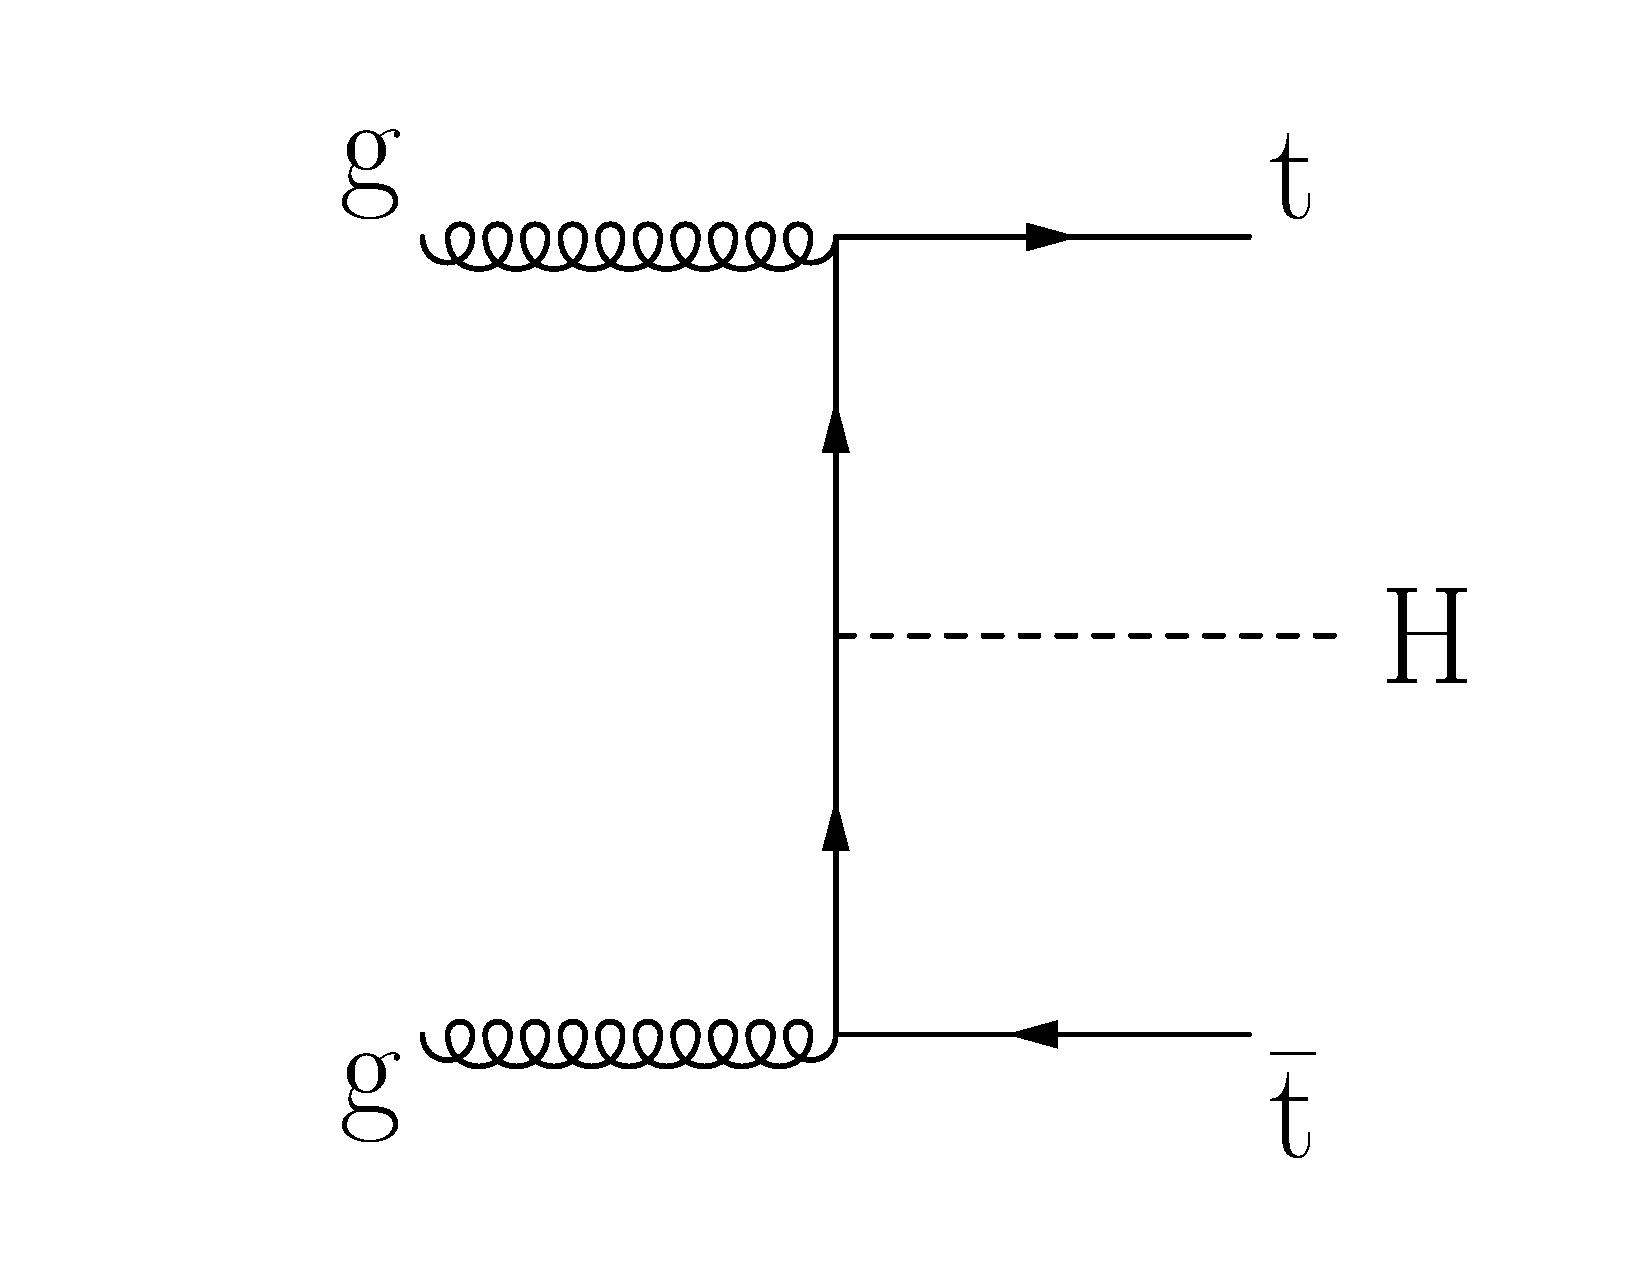
\includegraphics[width=0.45\textwidth]{Fig/ttH_Feynman_1.pdf}
	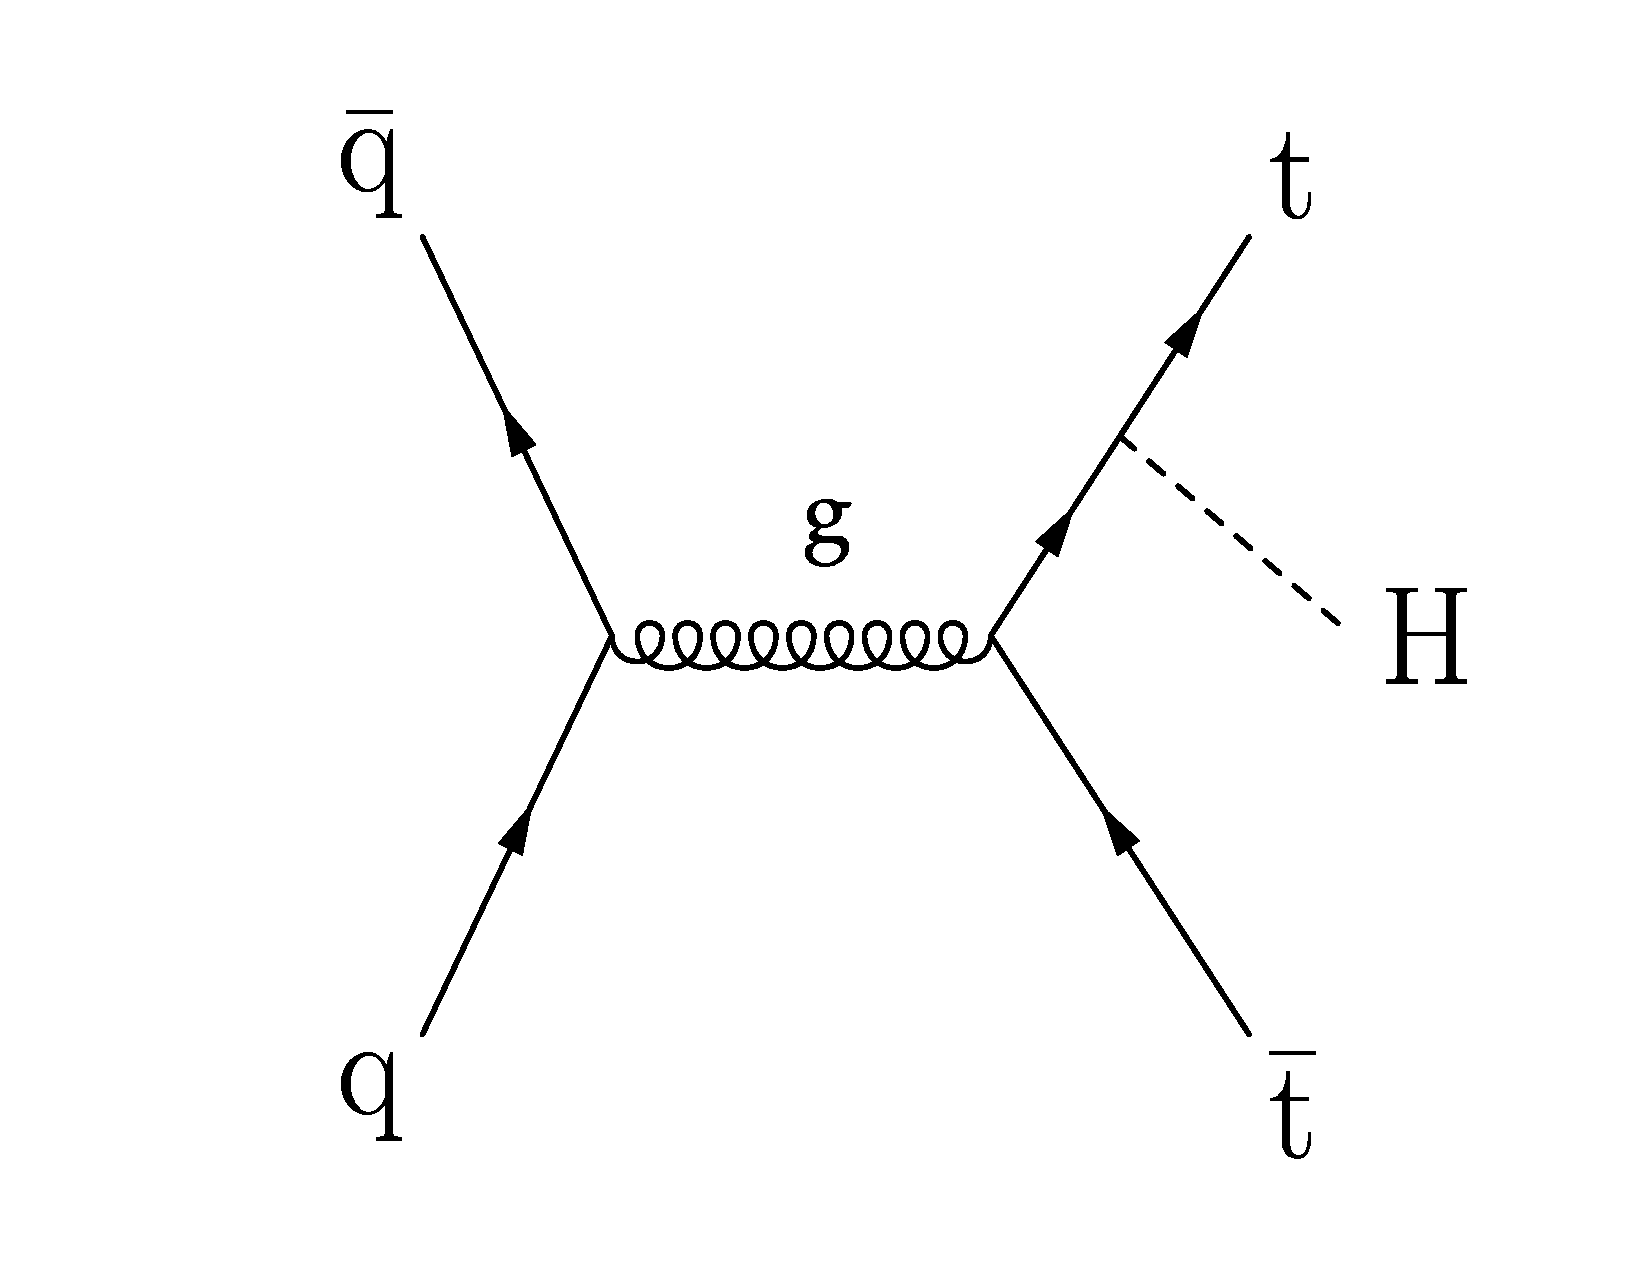
\includegraphics[width=0.45\textwidth]{Fig/ttH_Feynman_2.pdf}
	\caption{Few representative Feynman diagrams for the $\ttH$ production process. There are other diagrams also.}
	\label{ttH_feynman}
\end{figure}
Few of the leading order (LO) Feynman diagrams for \PH boson production in association with a pair
of top quarks ($\ttH$) are shown in Figure \ref{ttH_feynman}. In this analysis we have the following decay chains of top quark and Higgs:\\
\begin{equation}
\begin{split}
	&pp \to\ttH+X\\
	&\PQt \to\PW\PAQb, \PW\to \mathrm{qq'},\\
	%$\PH\to\PGt\PGt\to\tauh\ell\PGnGt\PGn_{\ell}$
	&\begin{tikzpicture}[node distance=0.5cm]
	\node (A) at (0, 2) {\PH};
	\node (B) at (1, 2) {$\PGt$};
	\node (E) at (1.25, 2) {$\PGt$};
	\node (C) at (2.5, 2) {$\tauh\PGnGt$};
	\node (D) at (2.5, 1.5) {$\ell\PGn_{\ell}\PGnGt$};
	\draw[->] (A) -- (B);
	\draw[->] (E) -- (C);
	\draw[->, to path={|- (\tikztotarget)}]
	(B) edge (D);
	\end{tikzpicture}
\end{split}
\end{equation}


Here \tauh collectively represents hadrons from \PGt decay. This particular channel has highest signal yields among all the channels that involve at least one \tauh in the final state. But at the same time it also suffers due to huge background contribution. However, overall in this channel we expect to get comparable sensitivity as that of the other categories.  


\subsection{Event selection}
The $1\ell + 1\tauh$ category targets $\ttH$ signal events in which the two top quarks decay hadronically and the \PH boson decays into two $\PGt$ leptons, one of which decays hadronically (denoted by \tauh, where \tauh denotes multiple pions) while the other one decays leptonically ($\uptau\to\ell\PGn_{\ell}\PGnGt$). Events selected in this category must contain one electron or muon and one $\tauh$ passing the medium Working Point (WP) (\tauh identification efficiency is 70\%, where as 2\% misidentification probability against jets) of the $\tauh$ identification discriminant. The lepton is required to be within the geometric acceptance of the lepton+\tauh cross-trigger, i.e. $|\eta| < 2.1$, and to have $\pt \geq 30$ \GeV ($ \geq 25$ \GeV) if it is an electron (muon). We further require that the $\tauh$ satisfies the condition $\pt \geq 30$ \GeV and that the event contains at least four jets with $\pt \geq 25$ \GeV and $|\eta| < 2.4$, among which at least two pass the loose selection criteria (92\% b-tagging efficiency and 10\% misidentification rate for light quark jets) of the \PQb-tagging algorithm or at least one passes the medium criteria (80\% b-tag efficiency and 1\% misidentification rate for light quark jets). Events with more than one electron or muon passing the tight object selection criteria or more than one loose \tauh passing the medium WP of the \tauh identification discriminant are vetoed to avoid overlap with the other categories.


\subsection{Background estimation}
Major background processes are taken into consideration in this analysis. Each background is categorised as either “reducible” or “irreducible” according to the source of the reconstructed and selected leptons. For all processes, a lepton is considered prompt if it originated from the decay of either a \PW boson, a \PZ boson or a $\PGt$ lepton. A background is considered reducible if one or more of the reconstructed electrons or muons or $\tauh$ passing the object selection criteria does not originate from a prompt electron, muon or $\tauh$. The main ``irreducible'' background contribution comes from inclusive $\ttbar$ production, as the topology of this process is similar to that of the signal process. Apart from these backgrounds, other contributing processes are inclusive production of Drell-Yan, $\ttbar\PZ$, $\ttbar\PW$, $\PW\PZ$, $\PZ\PZ$ and some other rare processes. All the ``irreducible'' backgrounds are estimated from Monte-Carlo (MC) simulation.\\
The dominant source of ``reducible'' background is from the events where a jet is misidentified as a lepton or $\tauh$, which is also called ``Fake'' background. This background is estimated in a data driven way which is described in the Section \ref{fake_bkg}.

\subsubsection{Estimation of the “Fake” background}\label{fake_bkg}
The background from misidentified leptons and $\tauh$ is estimated using the misidentification
probability (MP) method \cite{CMS:2018fdh}. The method is based on selecting a sample of events in an application region (AR), where the events satisfy all selection criteria of the SR, except that the electrons, muons, and $\tauh$ are required to pass relaxed selections instead of the nominal ones.
Events in which all leptons and $\tauh$ satisfy the nominal selections are vetoed, to avoid overlap with the Signal Region (SR). An estimate of the background from misidentified leptons and $\tauh$ in the SR is obtained by applying suitably chosen weights to the events selected in the AR. The weights, denoted by the symbol $w$, are given by the expression:
\begin{equation}
	w = (-1)^{n+1}\prod_{i=1}^{n}\frac{f_{i}}{1-f_{i}}
\end{equation}
where the product extends over all electrons, muons, and $\tauh$ that pass the relaxed criteria, but fail the nominal selection criteria, and `n' refers to the total number of such leptons and $\tauh$. The symbol $f_{i}$ denotes the probability for an electron, muon, or $\tauh$ passing the relaxed selection to also satisfy the nominal one. The contributions of irreducible backgrounds to the AR are subtracted based on the MC expectation of such contributions.\\
The probabilities $f_{i}$ for leptons are measured in multi-jet events, separately for electrons and muons, and are binned in $\pt$ and $\eta$ of the lepton candidate. The measurement is based on
selecting events containing exactly one electron or muon that passes the relaxed selection and
at least one jet separated from the lepton by $\DR > 0.7$. Selected events are then subdivided into “pass” and “fail” samples, depending on whether the lepton candidate passes the nominal selection or not. The fail sample is dominated by the contribution of multi-jet events. The
contributions of other processes are subtracted using MC.\\
The probabilities $f_{i}$ for $\tauh$ are determined as a function of $\pt$ and $\eta$ of the $\tauh$ candidate in a region enriched in $\ttbar$ +jets events containing a reconstructed opposite-sign electron-muon pair and at least two loose \PQb-tagged jets in addition to the $\tauh$ candidate. Contributions of genuine $\tauh$ are modelled using the MC simulation and subtracted.


\subsection{Search strategy}
In the $1\ell+1\tauh$ category a single BDT (Boosted Decision Tree) is trained to separate the $\ttH$ signal from the sum of the backgrounds. The background processes used for training are inclusive $\ttbar\PW$, $\ttbar\PZ$, $\ttbar$ and DY events. The BDTs take input variables related to the object multiplicities, the jet \PQb-tagging score, the flavor of the leptons, some basic kinematic properties of the objects, geometrical relations between the objects, the Hadronic Top Tagger score and other global variables. The jets that have not entered the computation of the hadronic top are used to reconstruct a second hadronic top, which also enters as input to the BDTs in these categories. In the same categories we also make use of the ``Secondary Vertex Fit'' mass of the leading $\ell+\tauh$   collection pair, as introduced by the $gg\to\PH\to\PGt\PGt$ analysis \cite{CMS:2014wdm}.\\
The choice of variables has been optimized according to their relative importance in terms of signal/background discriminating power. This variable ranking can be found in Figure \ref{var_rank} (left). The choice of the hyper-parameters used in the training has been done evaluating the ROC (receiver operating characteristic) curves and the expected limits. The ROC curves showing the separation of the $\ttH$ process from the rest of the backgrounds can be found in Figure \ref{var_rank} (right). Information on the choice of hyper-parameters can be are mentioned in this figure.
\begin{figure}[!htb]
	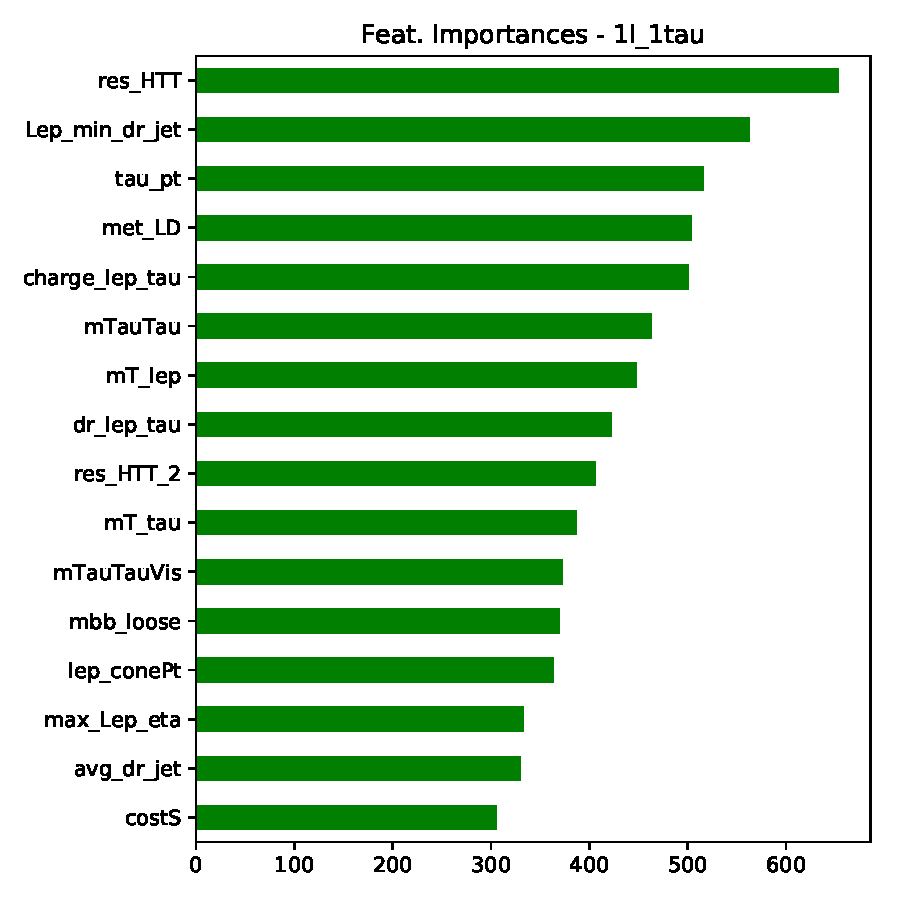
\includegraphics[width=0.45\textwidth]{Fig/var_rank.pdf}
	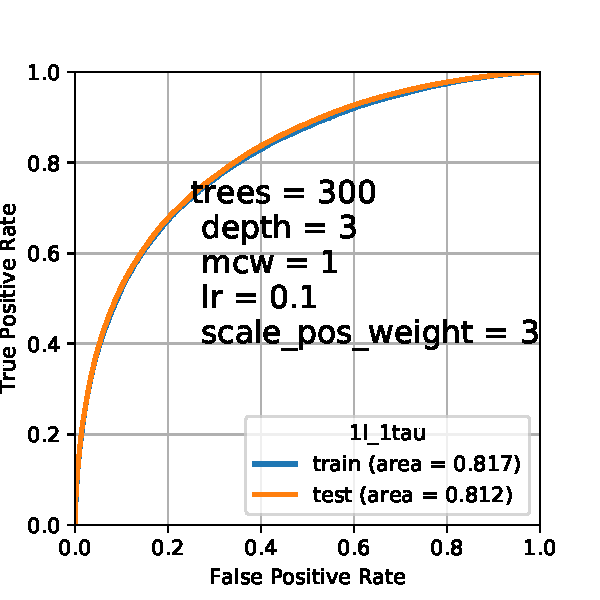
\includegraphics[width=0.45\textwidth]{Fig/roc.pdf}
	\caption{BDT Variable rankings (left) and ROC curve (right) for the $1\ell+1\tauh$ category}
	\label{var_rank}
\end{figure}

\subsection{Systematics}
The event rates and the distributions of the discriminating observables used for signal extraction may be altered by several experiment- or theory-related effects, referred to as systematic
uncertainties. Summary of the main sources of systematic uncertainty and their impact on the measurement of the $\ttbar\PH$ signal rate $\mu_{\ttbar\PH}=\frac{\text{No. of observed events}}{\text{Expected signal+bkg events}}$ are given in Table \ref{tab:nuissance_tth}.

\begin{table}[htb!]
	\caption{Impacts of different systematics on $\ttbar\PH$ signal rate.}
	\centering
	\begin{tabular}{|l|c|}
		\hline
		Source & $\Delta\mu_{\ttbar\PH}/\mu_{\ttbar\PH}$ \%\\
		\hline
		Trigger efficiency & 2.3\\
		\Pe, \PGm reconstruction and identification efficiency & 2.9\\
		\tauh identification efficiency & 4.6\\
		b tagging efficiency and mistag rate & 3.6\\
		Misidentified leptons and & 6.0\\
		Jet energy scale and resolution & 3.4\\
		MC and side-band statistical uncertainty & 7.1\\
		Theory-related sources & 4.6\\
		Normalization of MC-estimation processes & 13.3\\
		Luminosity & 2.2\\
		Statistical uncertainty & 20.9\\
		\hline
	\end{tabular}
	
	\label{tab:nuissance_tth}
\end{table}

\subsection{Results}
The production rates of the $\ttbar\PH$ signals are determined through a binned simultaneous
Maximum Likelihood fit to the output of the BDT as shown in Figure \ref{fig:tth_BDT}. In this calculation all the background and signal uncertainties are modelled as nuisance parameters and profiled in the maximum likelihood fit. Final results are obtained by combining the yields from 2016, 2017 and 2018 which amounts to integrated luminosities of 35.9 $\text{fb}^{-1}$, 41.5 $\text{fb}^{-1}$ and 59.7 $\text{fb}^{-1}$. The measured production rates for the $\ttbar\PH$ signal amounts to $1.80_{-2.22}^{+2.20}$ for $1\ell+1\tauh$ category shown in Figure \ref{fig:best_fit} for several categories.
\begin{figure}[htb!]
	\begin{subfigure}[b]{0.5\textwidth}
	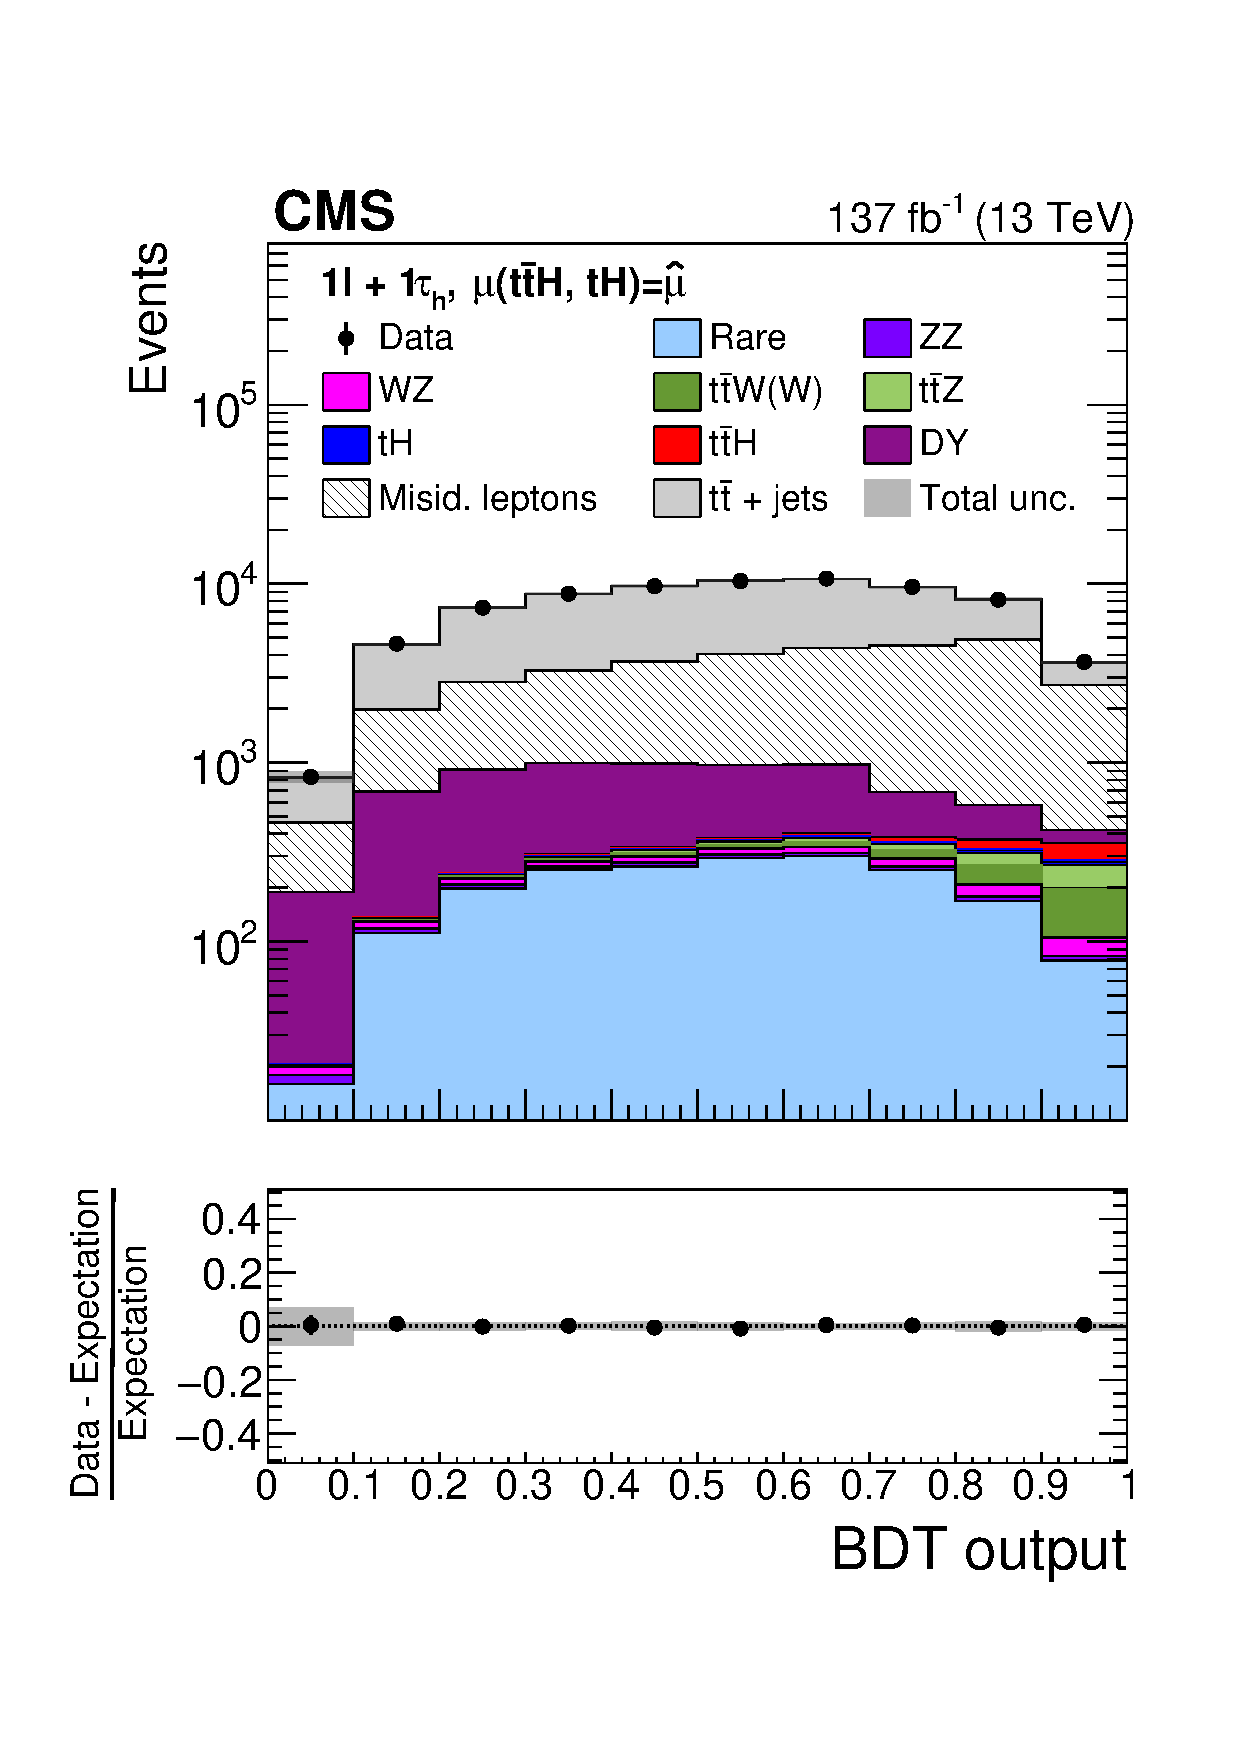
\includegraphics[width=0.9\textwidth]{Fig/Figure_010-a.pdf}
	\caption{BDT discriminator for $1\ell+1\tauh$ category}
	\label{fig:tth_BDT}
\end{subfigure}
\begin{subfigure}[b]{0.5\textwidth}
	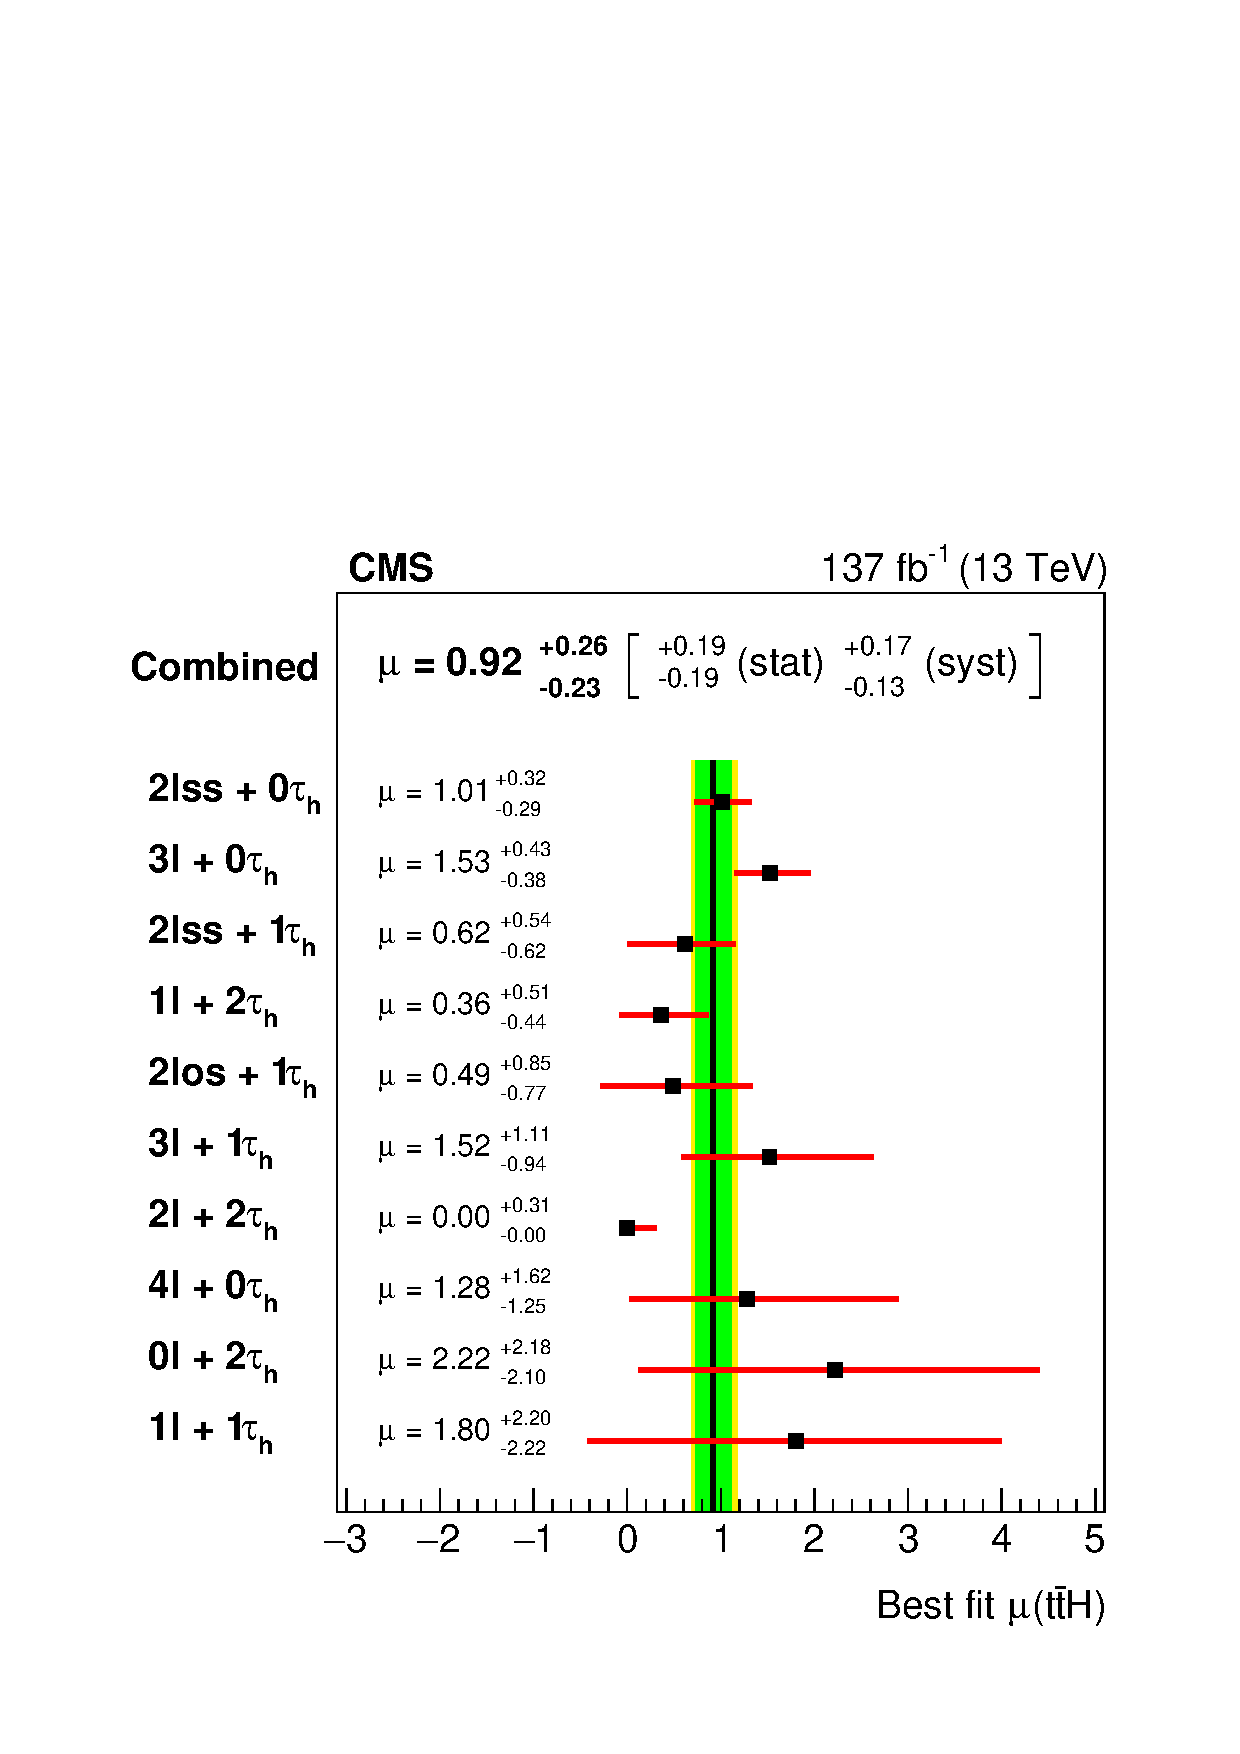
\includegraphics[width=0.9\textwidth]{Fig/Figure_013-a.pdf}
	\caption{Best fit value of $\ttbar\PH$ signal rate}
	\label{fig:best_fit}
\end{subfigure}	
\caption{BDT discriminator $1\ell+1\tauh$ category and the best fit value $\ttH$ signal}
\end{figure}

\subsection{My contribution to the analysis:}
In this analysis I was responsible for optimizing tau-Identification working point, b-tagging working point and other object selection criteria. Most importantly, I constructed the appropriate set of input variables for BDT that gives the best separation between signal and backgrounds. I have also performed the statistical checks and computed the final limit in this particular category. I also checked the feasibility of tagging boosted hadronically decaying top quark for this particular category.
%\clearpage

\section{Search for top squark pair production in a final state with two tau leptons in proton-proton collisions at $\sqrt{s} = 13$ TeV}\label{stop_search}

\subsection{Introduction}\label{susy_intro}

Supersymmetry (SUSY) \cite{Ramond:1971gb, Golfand:1971iw, Neveu:1971rx, Wess:1973kz, Fayet:1974pd, tHooft:1979rat, Kaul:1981hi, Nilles:1983ge, Martin:1997ns} is one of the most widely studied candidates of physics beyond the standard model (SM), providing solutions to various shortcomings of the SM. In SUSY models there is a bosonic supersymmetric partner (superpartner) for each fermion (and vice-versa), differing in 1/2 unit of spin and having the same other quantum numbers, as its SM partner. The superpartners of the SM gauge and Higgs bosons (gauginos and higgsinos, respectively) mix to produce charginos and neutralinos. The weakly interacting lightest neutralino \PSGczDo can be a dark matter candidate in $R$-parity conserving SUSY models~\cite{Farrar:1978xj}. The SUSY partners of left- and right-handed top quarks are the top squarks, \PSQtL and \PSQtR and can mix with each other, resulting in physical states \PSQtDo and \PSQtDt, with \PSQtDo defined to be the lighter of the two. The top squarks play an important role in stabilizing the Higgs boson mass by cancelling the dominant top quark loop correction. Therefore, there is a strong motivation to perform searches for top squark production.

In this study, we focus on the signal of top squark pair production in a final state with two tau leptons. This probes the part of the parameter space of the minimal supersymmetric standard model (MSSM) in which the lightest charginos (\PSGcpmDo) and neutralino preferentially couple to the third-generation fermions, such as tau lepton. The interaction of the charginos and neutralinos with fermion-sfermion pairs involves both gauge and Yukawa terms~\cite{Martin:1997ns}. If charginos and neutralinos are predominantly higgsino-like, they will preferentially couple to third-generation fermion-sfermion pairs through the large Yukawa coupling. Moreover, the Yukawa coupling to the tau lepton-slepton pairs can be large for a large value of $\tan\beta$ even if the higgsino component is relatively small. Additionally, a large value of tan$\beta$ can make the lighter state of the superpartner of the tau lepton ($\PSGtDo$) much lighter than the superpartners of the first and second generation leptons. Consequently, the chargino decays predominantly as $ \PSGcpDo \to \PSGtpDo \PGnGt $ or $ \PGtp \PSGnGt $ (charge conjugation is assumed throughout in this document), and the decay rates in the electron and muon channels are greatly suppressed~\cite{Baer:1997yi, Guchait:2002xh}.
Therefore, searches for SUSY signals in electron and muon channels are less sensitive to this scenario, and \PGt-rich final states are expected in SUSY cascade decays.

\subsection{The signal process}

We focus on the cascade top squark decays
$\PSQtDo \to \PQb \PSGcpDo \to \PQb \PSGtpDo \PGnGt \to  \PQb \PGtp \PSGczDo \PGnGt$
 ~and~
$\PSQtDo \to \PQb \PSGcpDo \to \PQb \PGtp \PSGnGt \to \PQb \PGtp \PSGczDo \PGnGt$.
The \PSGczDo is assumed to be the lightest SUSY particle (LSP). Being neutral and weakly interacting, it leaves no signature in the detector, resulting in an imbalance in transverse momentum \pt. The neutrinos produced in the decay chains also contribute to the \pt imbalance.
Hence, the events of interest contain two tau leptons, two {\PQb} quarks, and a \pt imbalance.
The decay chains are depicted by the four diagrams in Figure~\ref{fig:sigFeyn} within the simplified model spectra (SMS) framework~\cite{Alwall:2008ag, Alves:2011wf}. It is assumed that the $\PSGcpDo$ decays to \PSGtpDo or \PSGnGt with equal probability. So each diagram contribute 25\% to the signal process. The masses of SUSY particles appearing in the decay chain are
determined by the parametrization
\begin{equation}
	\begin{aligned}
	m_{\PSGcmDo} - m_{\PSGczDo} &= 0.5 \
	(m_{\PSQtDo} - m_{\PSGczDo} ) ,
	\\
	m_{\PSGt_{1}} - m_{\PSGczDo} &= x \
	(m_{\PSGcmDo} - m_{\PSGczDo} ) ,
	\\
	x &\in [0.25,\ 0.5,\ 0.75] ,
	\\
	m_{\PSGnGt} & = m_{\PSGt_{1}} .
	\end{aligned}
	\label{eq:mass}
\end{equation}

\begin{figure}[!htbp]
	\centering
	
	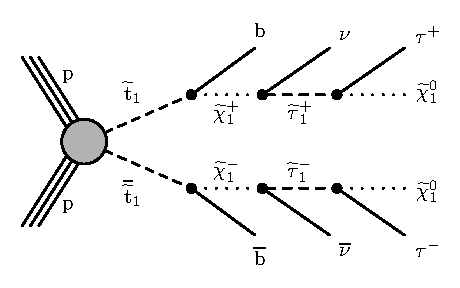
\includegraphics[width=0.45\textwidth]{Fig/Figure_001-a.pdf}
	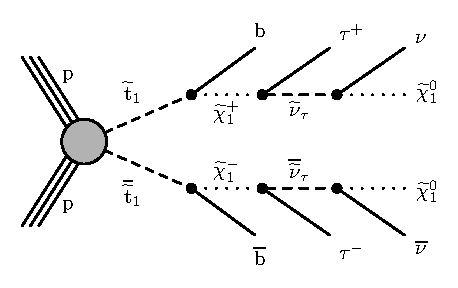
\includegraphics[width=0.45\textwidth]{Fig/Figure_001-b.pdf} \\
	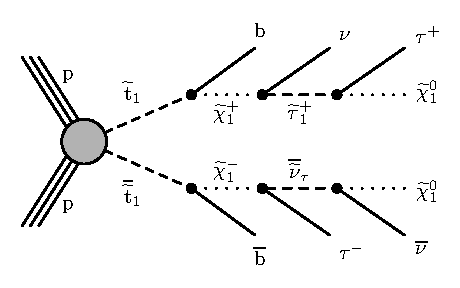
\includegraphics[width=0.45\textwidth]{Fig/Figure_001-c.pdf}
	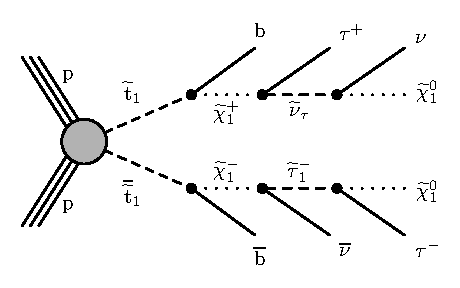
\includegraphics[width=0.45\textwidth]{Fig/Figure_001-d.pdf}
	
	%\setcounter{figure}
	\caption{Top squark pair production in proton-proton collisions at the LHC, producing pairs of \PQb quarks and taus accompanied by neutrinos and LSPs in the final state.
	}
	\label{fig:sigFeyn}
\end{figure}

\subsection{Why \PGt lepton final state}
The top squark search in CMS has been already performed in electron and muon final states. But we are interested in \PGt-lepton final state because of the following reason.\\
The charginos ($\PSGc_{i}^{\pm}$) and neutralinos ($\PSGc_{i}^{0}$) are admixtures of gauginos and higgsinos given by:
\begin{equation}
\begin{aligned}
	\PSGc_{i}^{\pm}&=C_{1i}\PSWpm + C_{2i}\PSH^{\pm} ~~~~~~~~~~~~~~~~~~~~~~~~~~~~\text{with}~i\in[1,2]\\\
	\PSGc_{i}^{0}&=N_{1i}\PSBz+N_{2i}\PSWz + N_{3i}\PSH_{u}^{0}+N_{4i}\PSH_{d}^{0}~~~~~ \text{with}~i\in[1,4]
	\end{aligned}
\end{equation}
The higgsino components of the charginos and neutralinos couple to the lepton-slepton pair as $M_{\ell}/\text{cos}\beta$. So in the higgsino like scenario ($|C_{2i}|^{2}\gg |C_{1i}|^{{2}}$ and $|N_{3i}|^{2}+|N_{4i}|^{2}\gg |N_{1i}|^{2}+|N_{2i}|^{2}$) and/or high tan$\beta$ scenario, the chargino most often decays to \PGt-leptons as $M_{\PGt}\gg M_{\PGm},M_{\Pe}$, leading to \PGt rich final state.\\
The search is already performed in di-\tauh final state \cite{CMS:2019lrh} with 2016 and 2017 data, where top squark mass up to 1100 \GeV for nearly massless neutralino was excluded. In this analysis main focus is given to the semileptonic categories where one \PGt decays hadronically and the other leptonically. The probability of two \PGt decaying hadronically is $\approx 42\%$. But if we consider the scenario where one \PGt decays hadronically and other leptonically, then that probability is also $\approx 40\%$. So one expect similar signal yields as that of the di-\tauh final state. Also triggering semileptonic final state is easier. This is the motivation for probing the semileptonic channels as well. Then these semileptonic channels are combined with the hadronic channel, to have the  result for entire Run2 dataset.

\subsection{Search Variables}
The signal event consists of one high \pt hadronically decaying $\PGt$ (\tauh) jets, one lepton ($\PGm$ or \Pe), a large amount of missing transverse momentum (\ptmiss), and at least one \PQb-tagged jet. The major sources of missing energy is from the weakly interacting neutralino (which can be massive), unlike the SM backgrounds. The missing energy is correlated with the visible objects, in particular the \tauh jets and leptons ($\PGm$ or \Pe). Consequently in the signal events, the correlation between visible and invisible parts is expected to be different in comparison to the SM background processes. This feature of the correlation can be exploited through the construction of a variable called the transverse mass, which is defined as.
\begin{equation}
\mT^{2}(\ptvec^{~\text{vis}},\ptvec^{~\text{inv}}) = m_{\text{vis}}^{2}+m_{\text{inv}}^{2}+2(\ET^{\text{vis}}\ET^{\text{inv}}-\ptvec^{\text{~vis}}.\ptvec^{\text{~inv}})
\label{eqn:mT}
\end{equation}

Generally, this variable carries information about the mass of parent of the visible ($m_{\text{vis}}$) and the invisible ($m_{\text{inv}}$) decay products. However, since there are multiple sources of missing momentum in the signal process, the appropriate variable which can render the parent particle masses is the ``stransverse mass'' \cite{Lester:1999tx, Barr:2003rg, Barr:2009wu},
\begin{equation}
\mTii(\ptvec^{\text{~vis1}}, \ptvec^{\text{~vis2}}, \ptmiss) = \min_{\ptvec^{~\text{inv1}}+\ptvec^{~\text{inv2}}=\ptvecmiss}[\max\{\mT(\ptvec^{~\text{vis1}},\ptvec^{~\text{inv1}}), \mT(\ptvec^{~\text{vis2}},\ptvec^{~\text{inv2}})\}]
\label{eqn:mt2}
\end{equation}
In Equation \ref{eqn:mt2}, since the momenta of the individual invisible particles is not known, the missing energy(\ptmiss) is divided into two components ($\ptvec^{~\text{inv1}}$ and $\ptvec^{~\text{inv2}}$) in such a way that the value of $\mTii$ is minimum. In our case $\mTii$ is computed using the \tauh and $\PGm/\Pe$ and \ptmiss. Then its upper limit in our signal will be at the chargino mass. This is different from the SM background processes. For example, in \ttbar events the upper limit is at the W boson mass. Since this is a search, when calculating $\mTii$ for the signal, the mass of the invisible particle in equation \ref{eqn:mt2} is set to zero as the neutralino mass is not known.

In addition, we construct another variable $\ST$, sum of the transverse momenta of the visible particles in the final-state,
\begin{equation}
\ST= \pt^{\PGm/\Pe}+\pt^{\tauh}+\sum_{jets}\pt
\label{eqn:sT}
\end{equation}
So finally we consider three search variables:
\begin{itemize}
	\item \ptmiss: Sensitive to the kinematics of the $\nu$ and \PSGczDo;
	\item $\mTii$: Sensitive to the mass of \PSGcpmDo;
	\item $\ST$: Sensitive to the total mass of the two top squarks.
\end{itemize}



\subsection{Search Region}
Signal events with different top squark and LSP masses populate different regions of the phase space. For example, regions with low $\ptmiss$, $\mTii$, and $\ST$ are sensitive to signals with low top squark masses. On the other hand, events with high $\ptmiss$, $\mTii$, and $\ST$ are sensitive to models with high top squark and low LSP masses. In order to obtain the highest sensitivity over the entire phase space, the signal region (SR) is divided into several bins as a function of the measured $\ptmiss$, $\mTii$ , and $\ST$. The optimization of the bins are performed by comparing the distributions of the variables between backgrounds and signals of different mass points, which can be seen in Figure \ref{fig:compare_shape}. Closely examining the sensitivities of the search variables, we divided the entire phase space into 15 bins. The bins are shown in Figure \ref{fig:SR_Bins}. 

\begin{figure}[htb!]
	\centering
	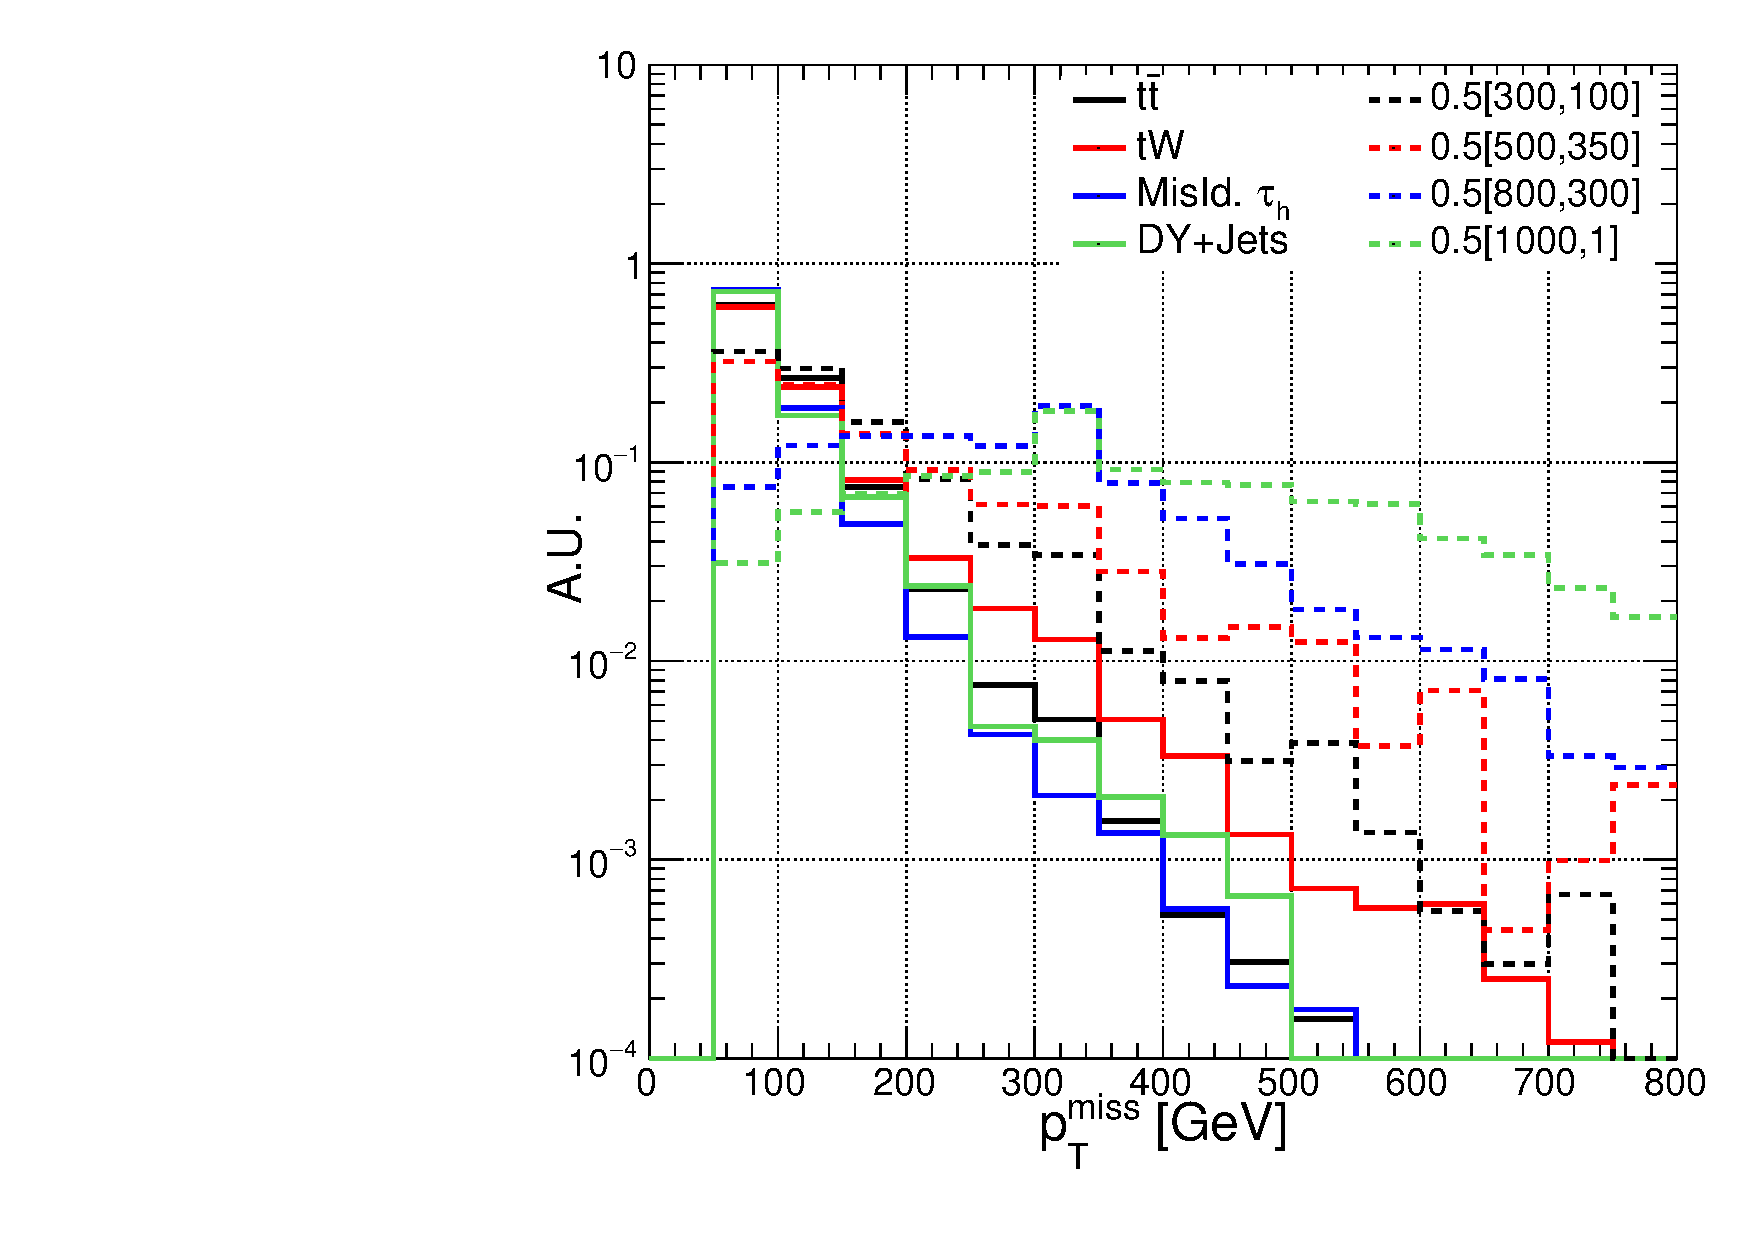
\includegraphics[width=0.32\textwidth]{Fig/met.pdf}
	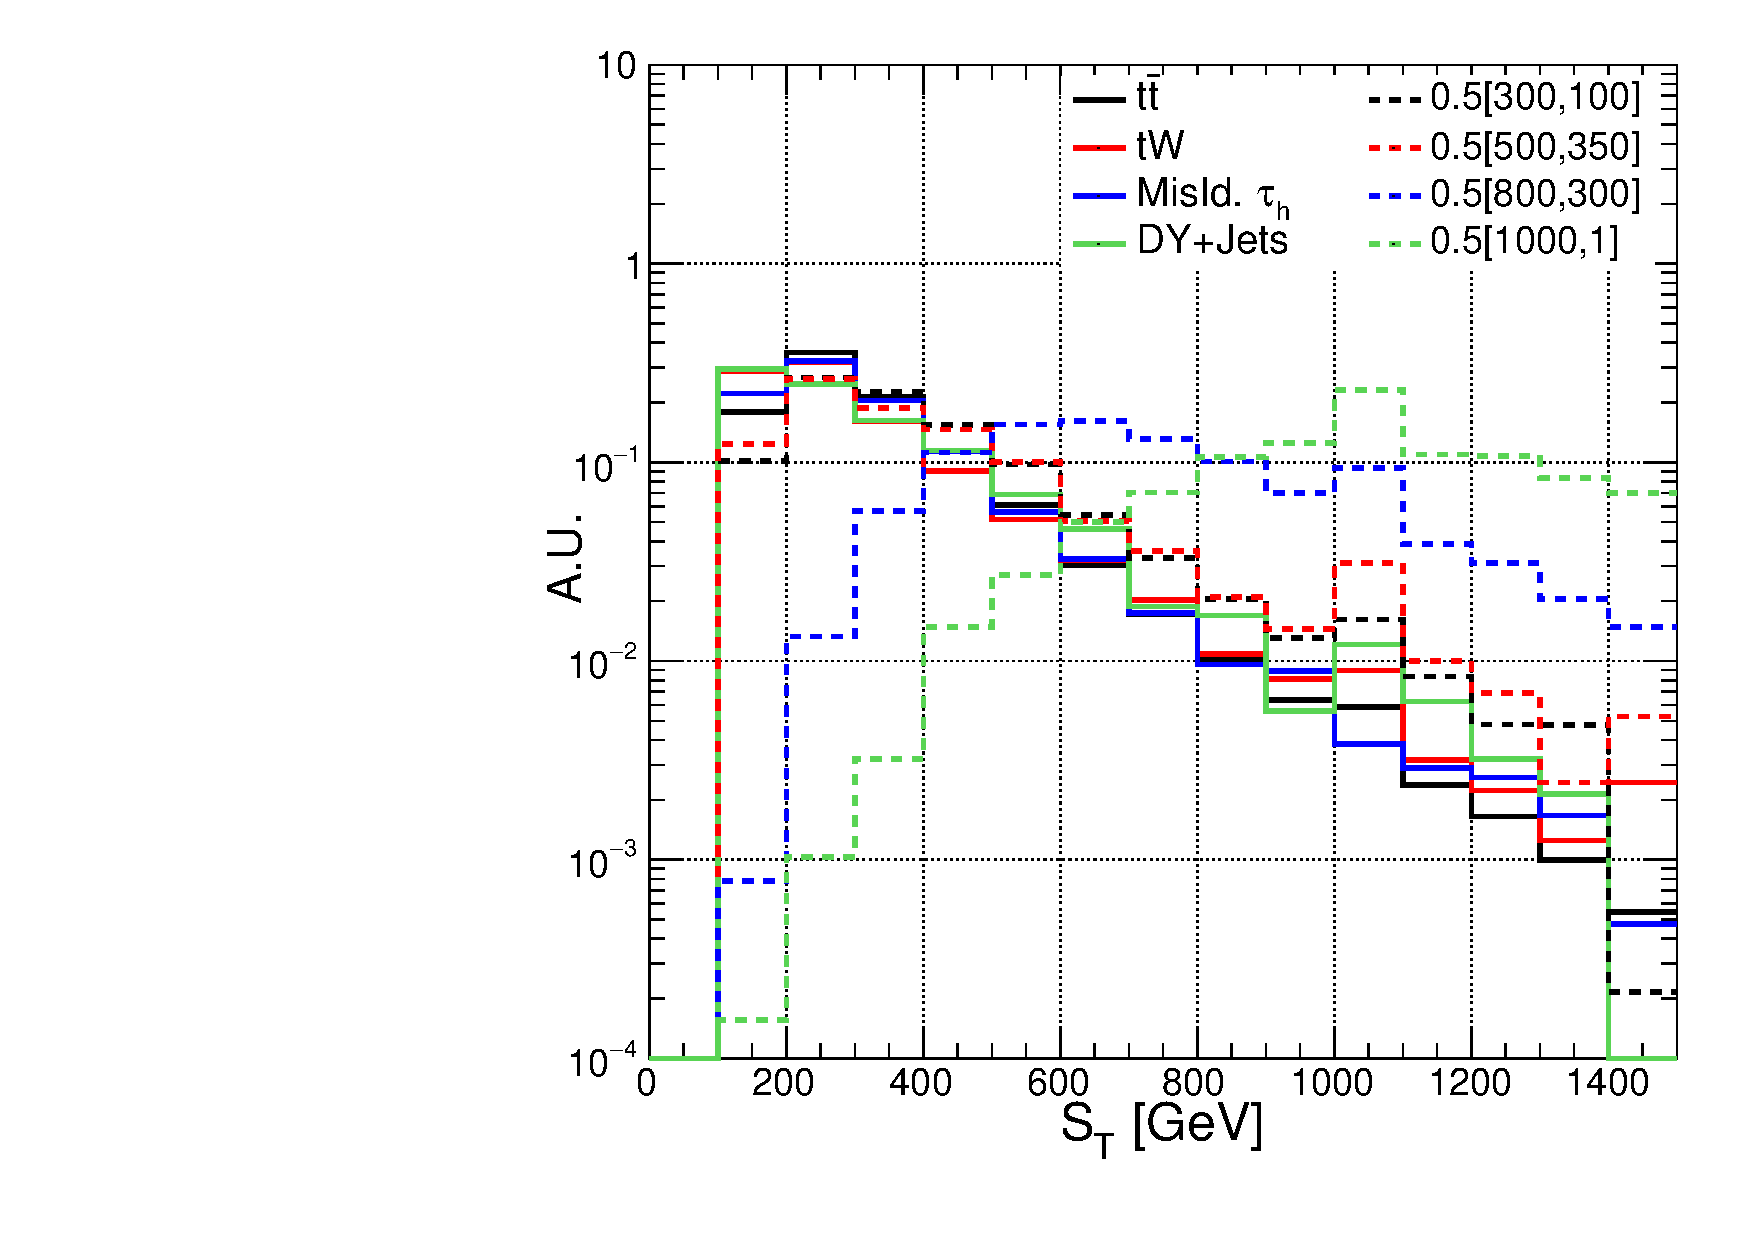
\includegraphics[width=0.32\textwidth]{Fig/ht.pdf}
		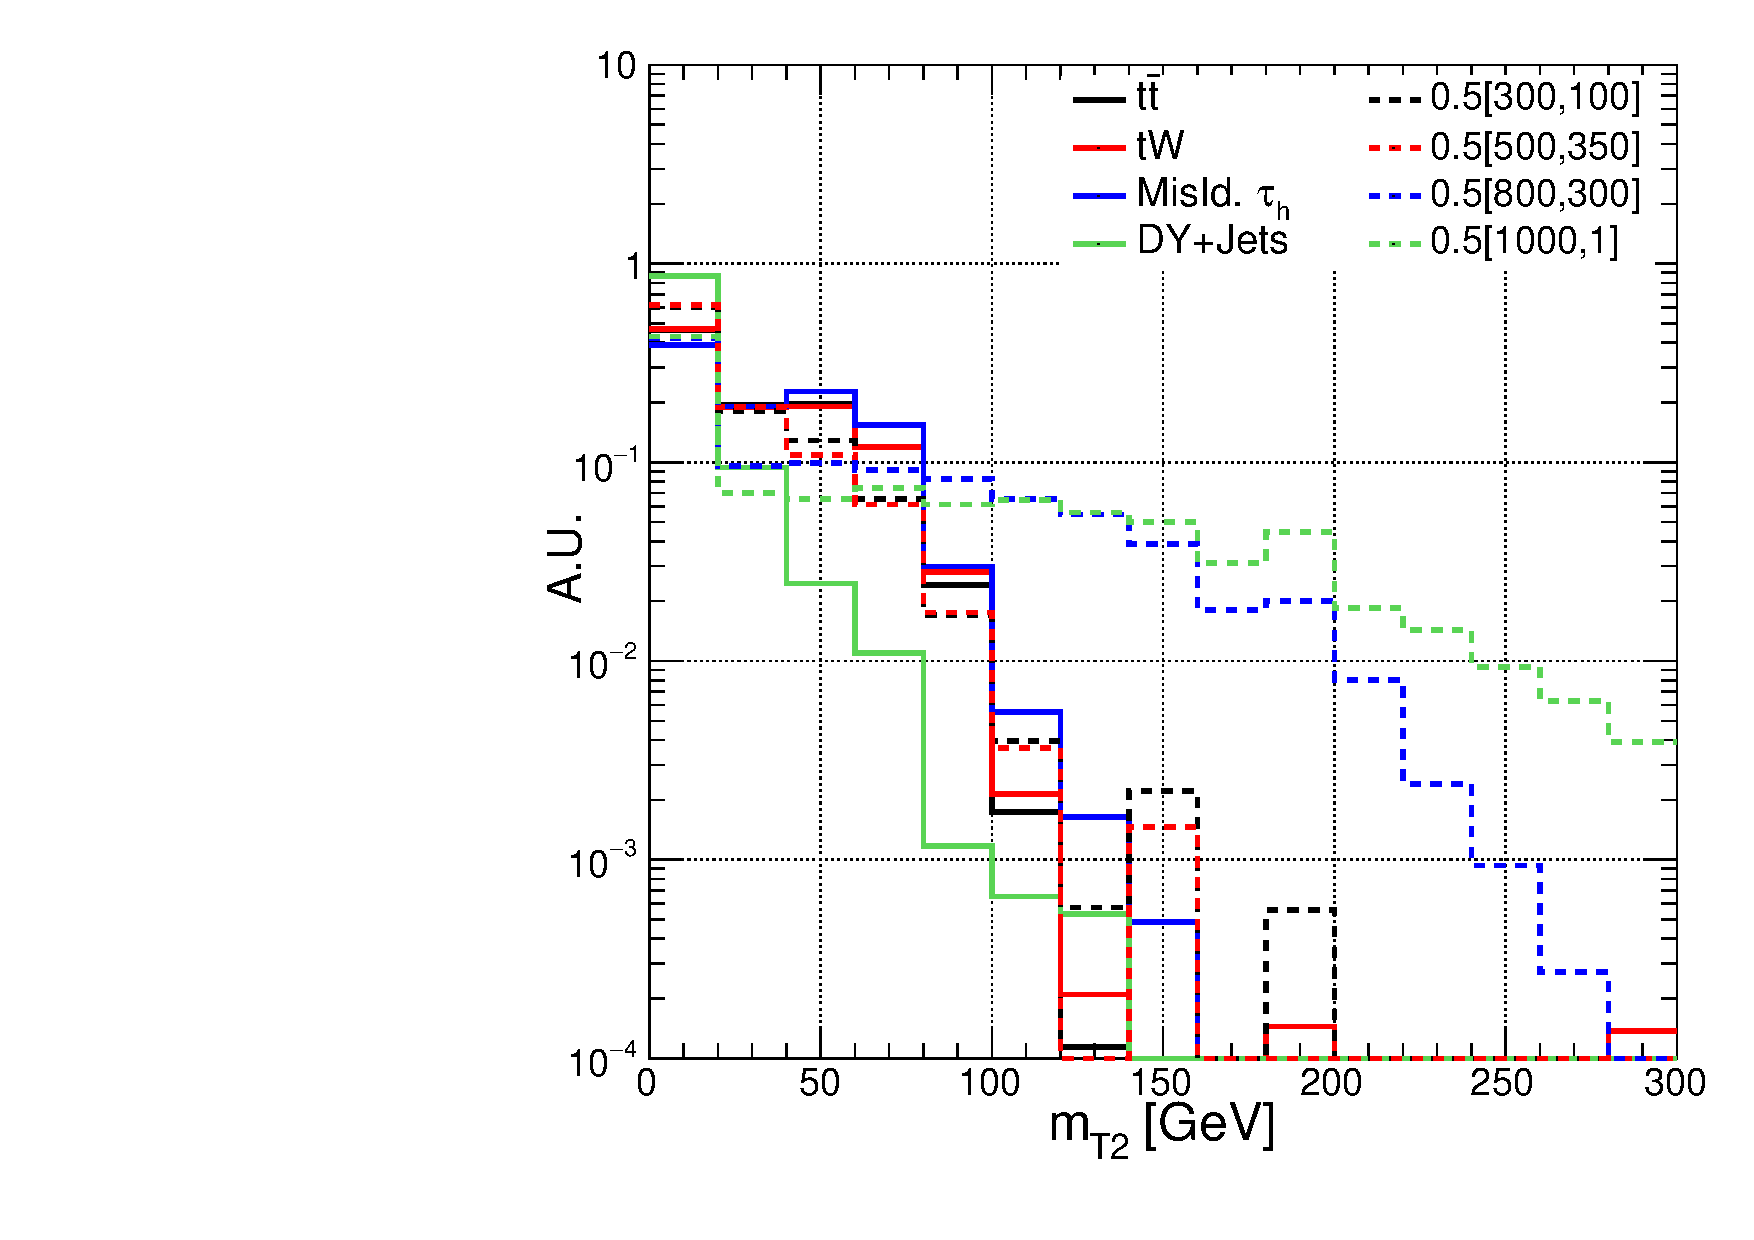
\includegraphics[width=0.32\textwidth]{Fig/mt2.pdf}
	\caption{A shape comparison of the search variables between signal, setting $x=0.5$, $m_{\PSQtDo},m_{\PSGcz}=(300,100),(500,350),(800,300),(1000,1)$ and backgrounds.}
	\label{fig:compare_shape}
\end{figure}
\begin{figure}[htb!]
	\begin{center}
		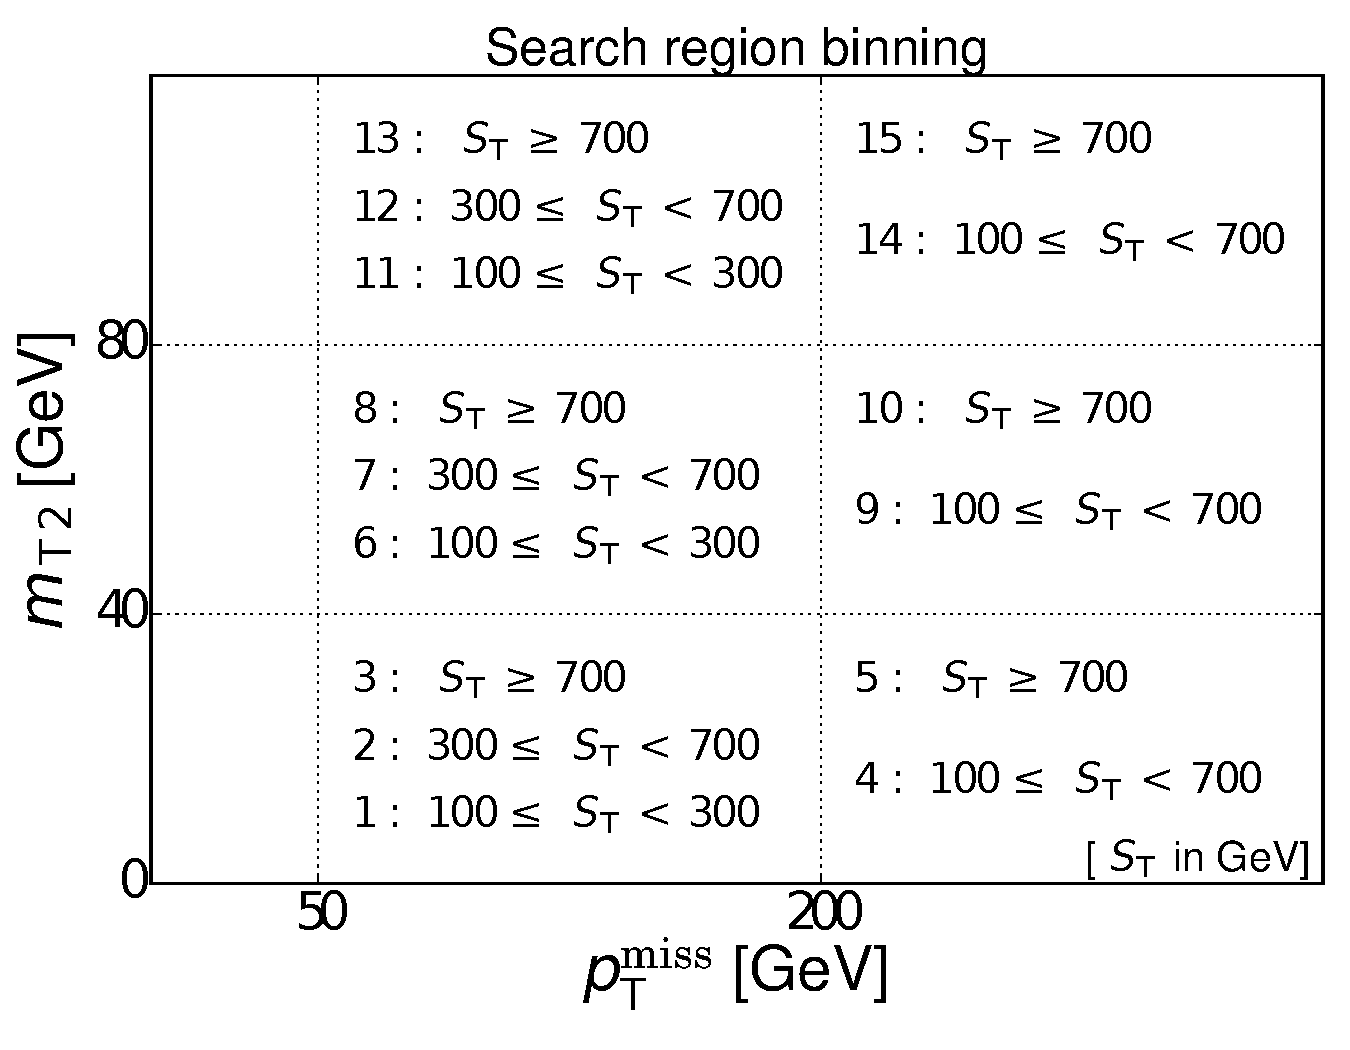
\includegraphics[width=0.6\textwidth]{Fig/sig_binning.pdf}
	\end{center}
	\caption{Subdivisions of the phase space in the signal region.}
	\label{fig:SR_Bins}
\end{figure}

\subsection{Signal Region Selection}
Signal events are selected using single muon (single electron) trigger for $\PGm\tauh$ ($\Pe\tauh$) channels. For offline selection we require \ptmiss$>50$ \GeV, \ST$>100$ \GeV and at least one b-tagged jet passing medium working point (WP) of the DeepJet b-tagging algorithm. For $\PGm\tauh$ category the events should have exactly one \PGm and exactly one \tauh of opposite sign. The \PGm should pass medium isolation WP and have $\pt>28$ \GeV and $|\eta|<2.4$. The \tauh should pass tight $\PGt$-identification WP and have $\pt>30$ \GeV and $|\eta|<2.3$.  Events with any extra lepton with \pt$>15$ \GeV and $|\eta|<2.4$ are vetoed to remove the overlap between different categories. The selection criteria for $\Pe\tauh$ category is similar to the $\PGm\tauh$ category, except from the fact that the electron should pass tight isolation WP and have $\pt>30~(36)$ \GeV for 2016 (2017 and 2018) and $|\eta|<2.1$. The Data-MC comparison for \ptmiss, \ST and \mTii are shown in the Figure \ref{fig:data_mc_comp}.
\begin{figure}[htb!]
	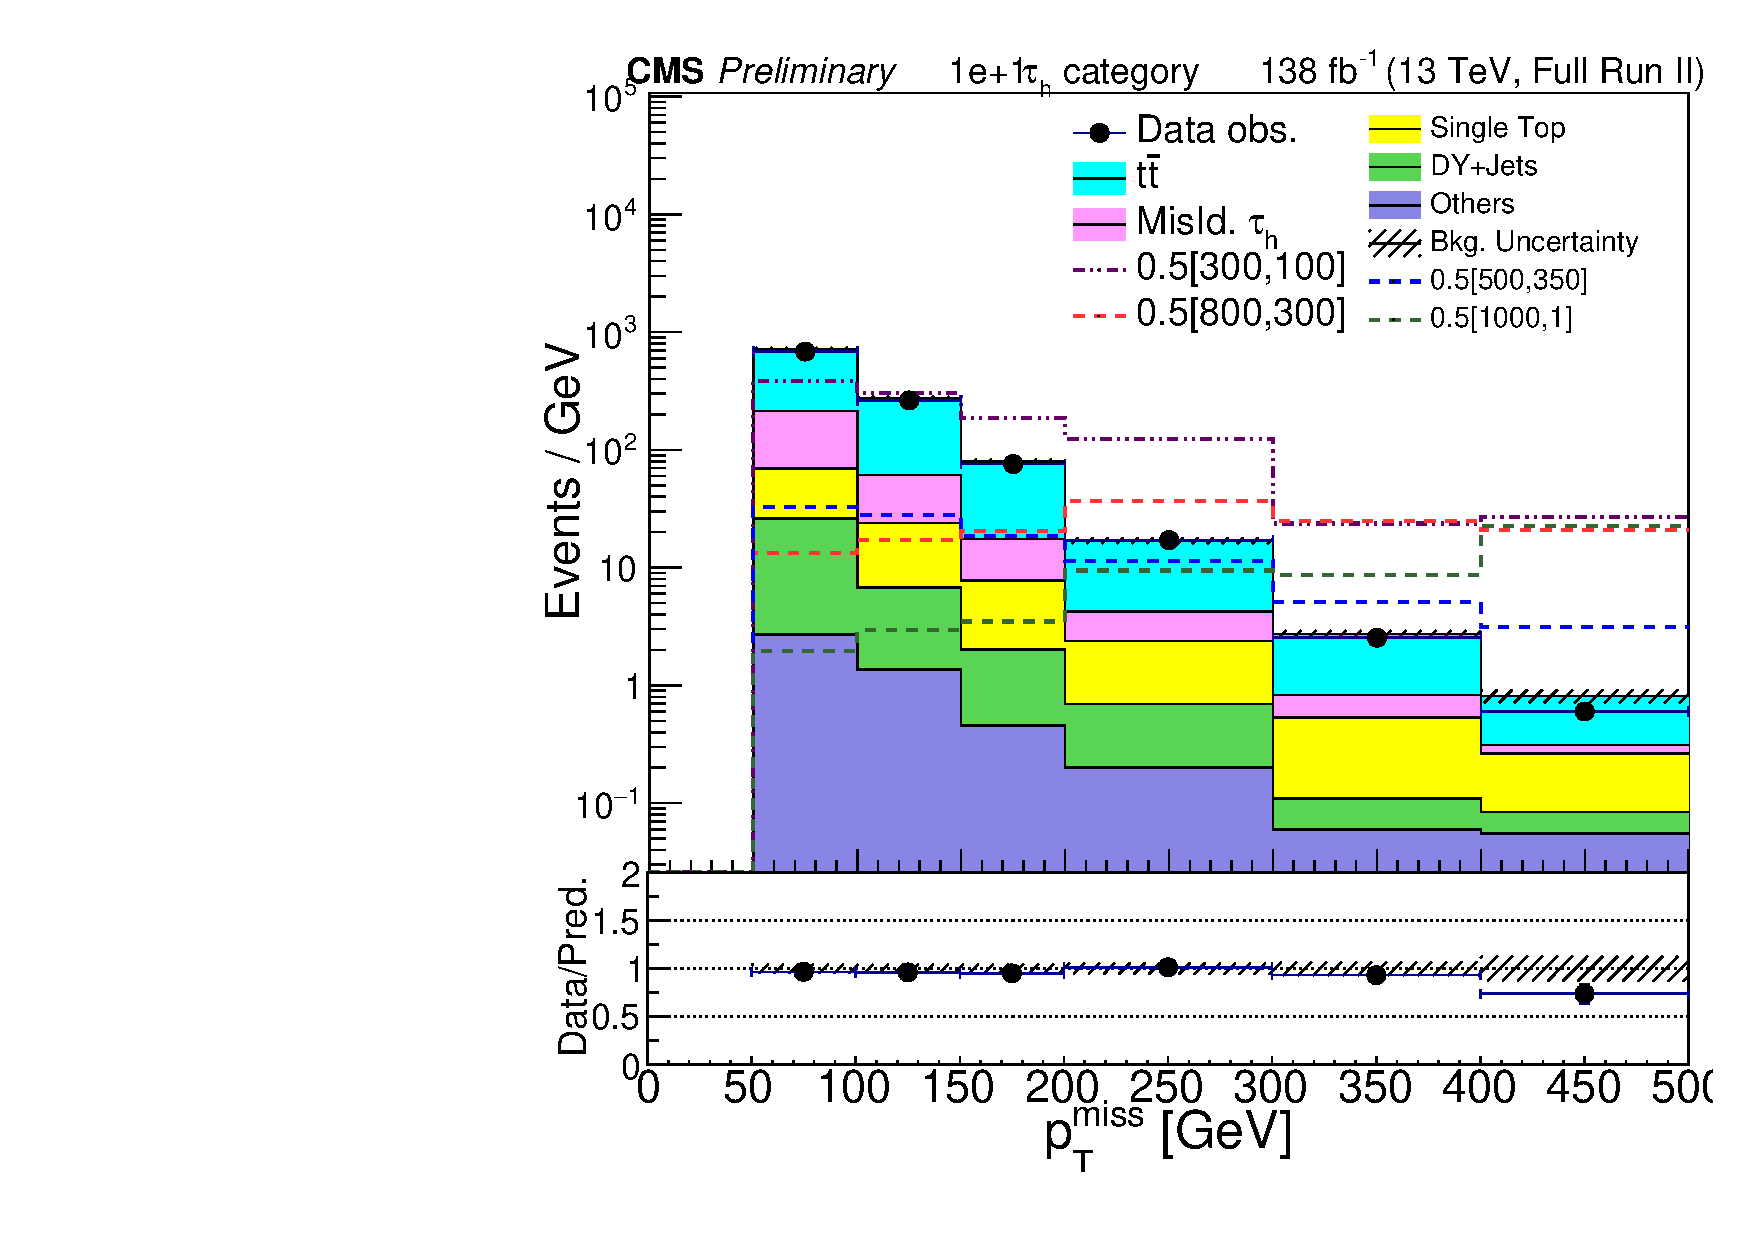
\includegraphics[width=0.32\textwidth]{Fig/Met_1E1Tau_FullRun2.pdf}
	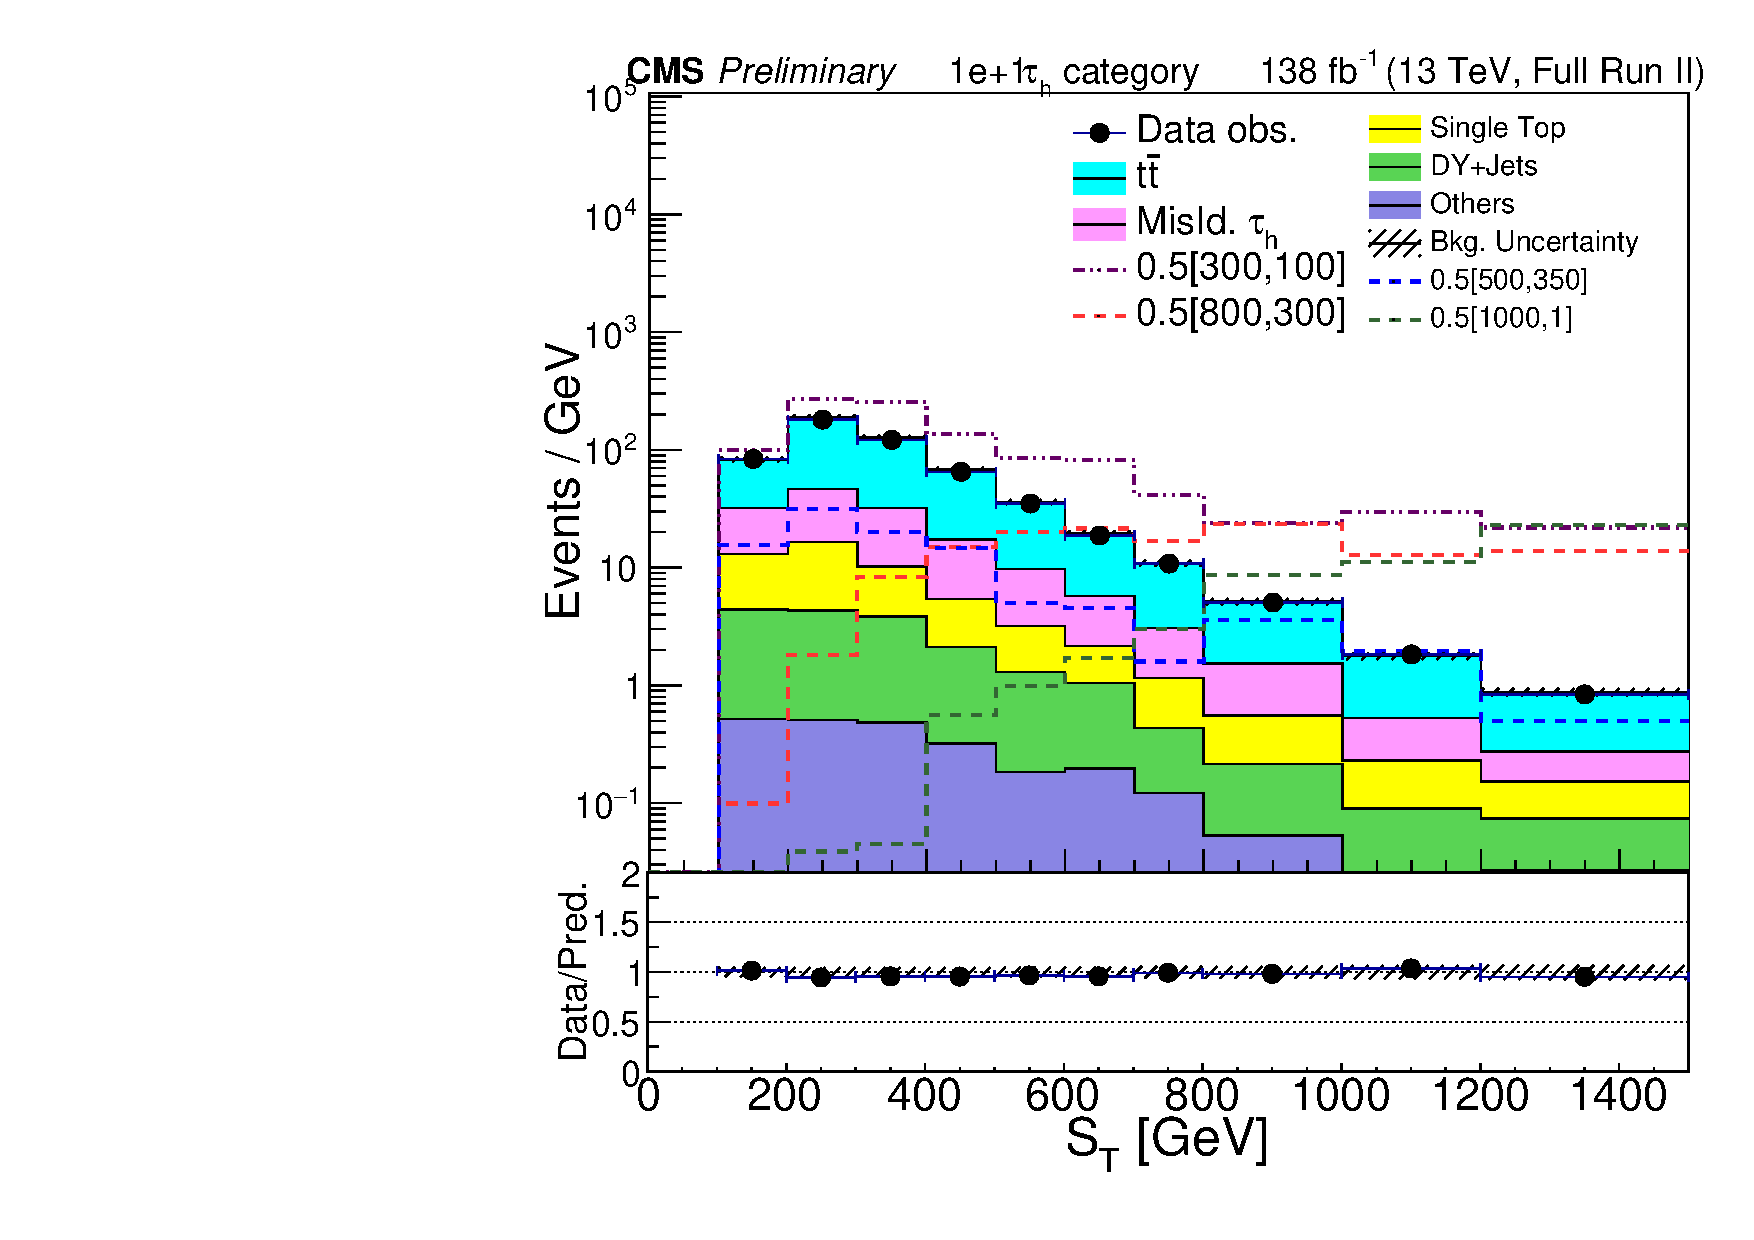
\includegraphics[width=0.32\textwidth]{Fig/Ht_1E1Tau_FullRun2.pdf}
	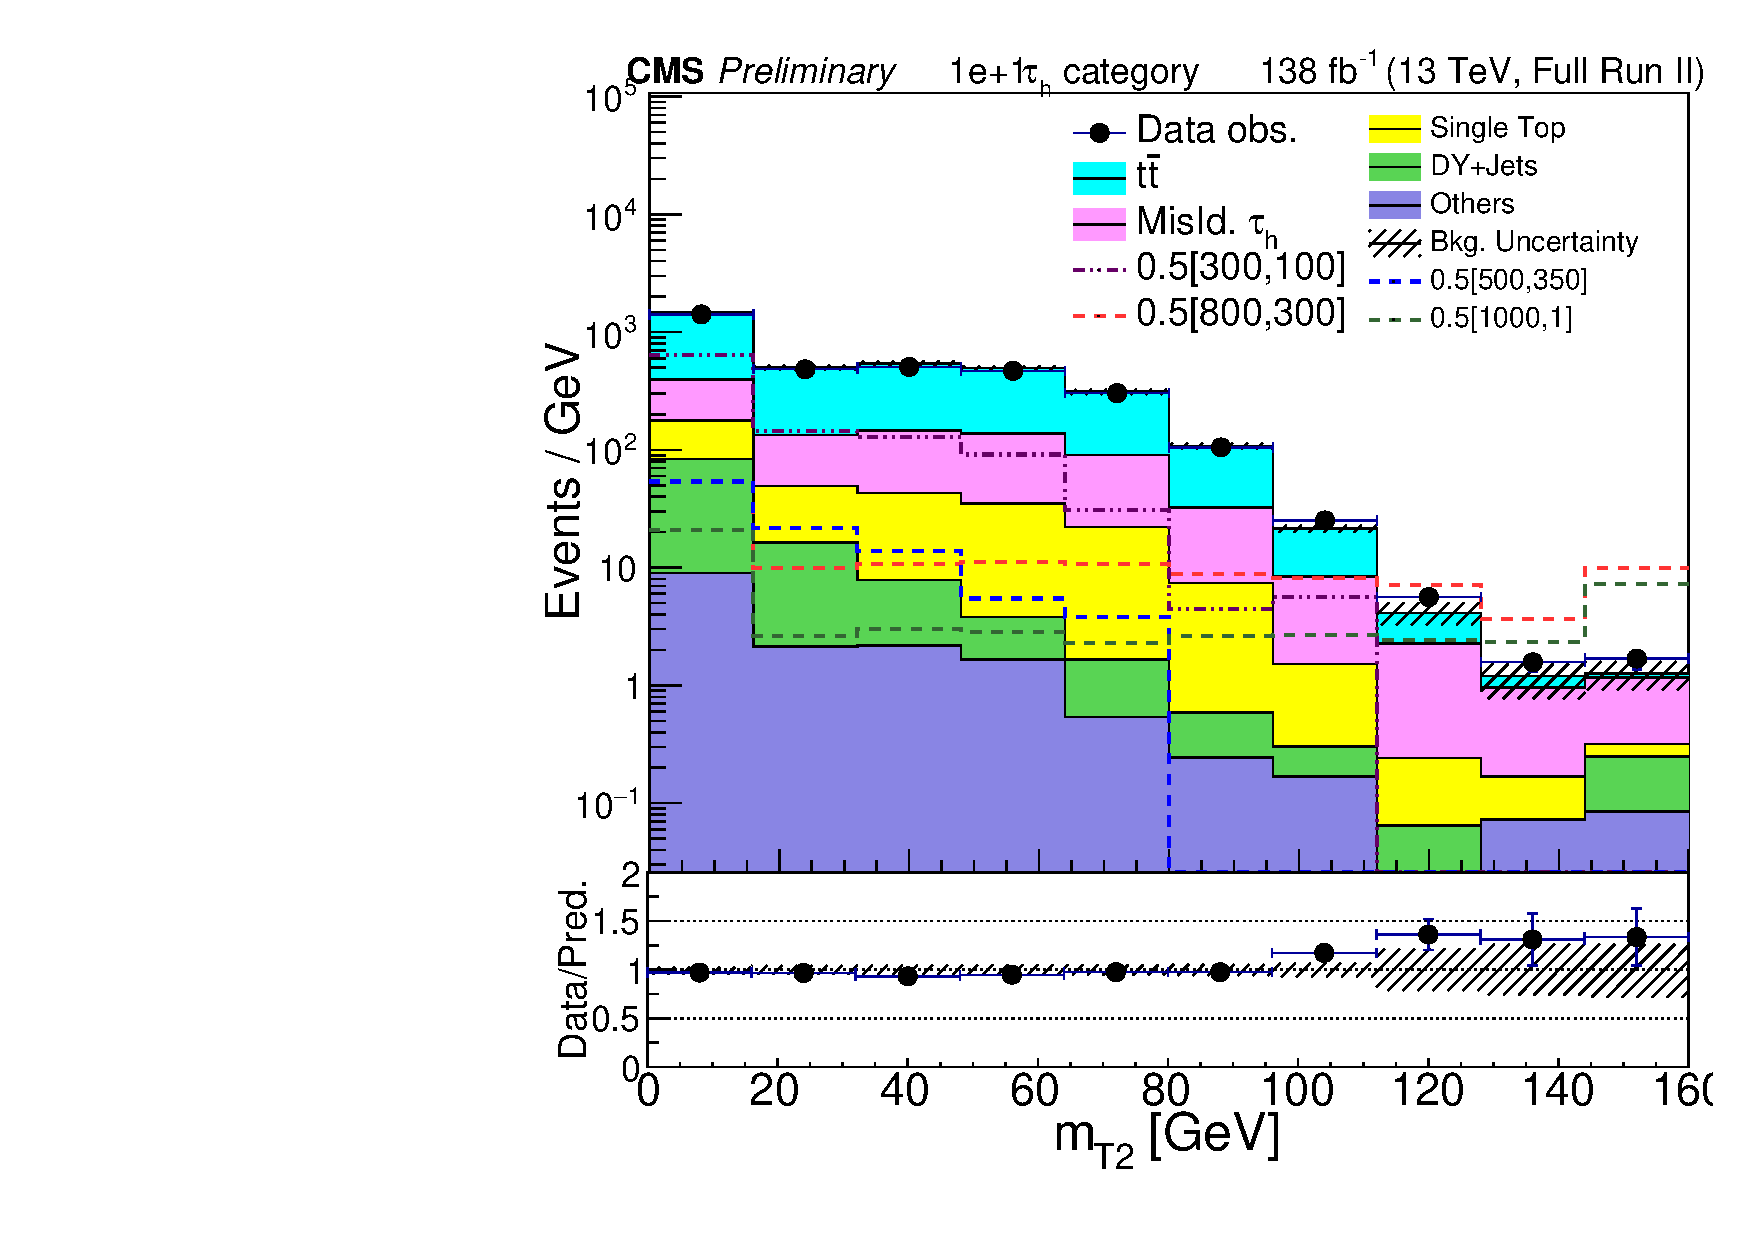
\includegraphics[width=0.32\textwidth]{Fig/Mt2_1E1Tau_FullRun2.pdf}\\
	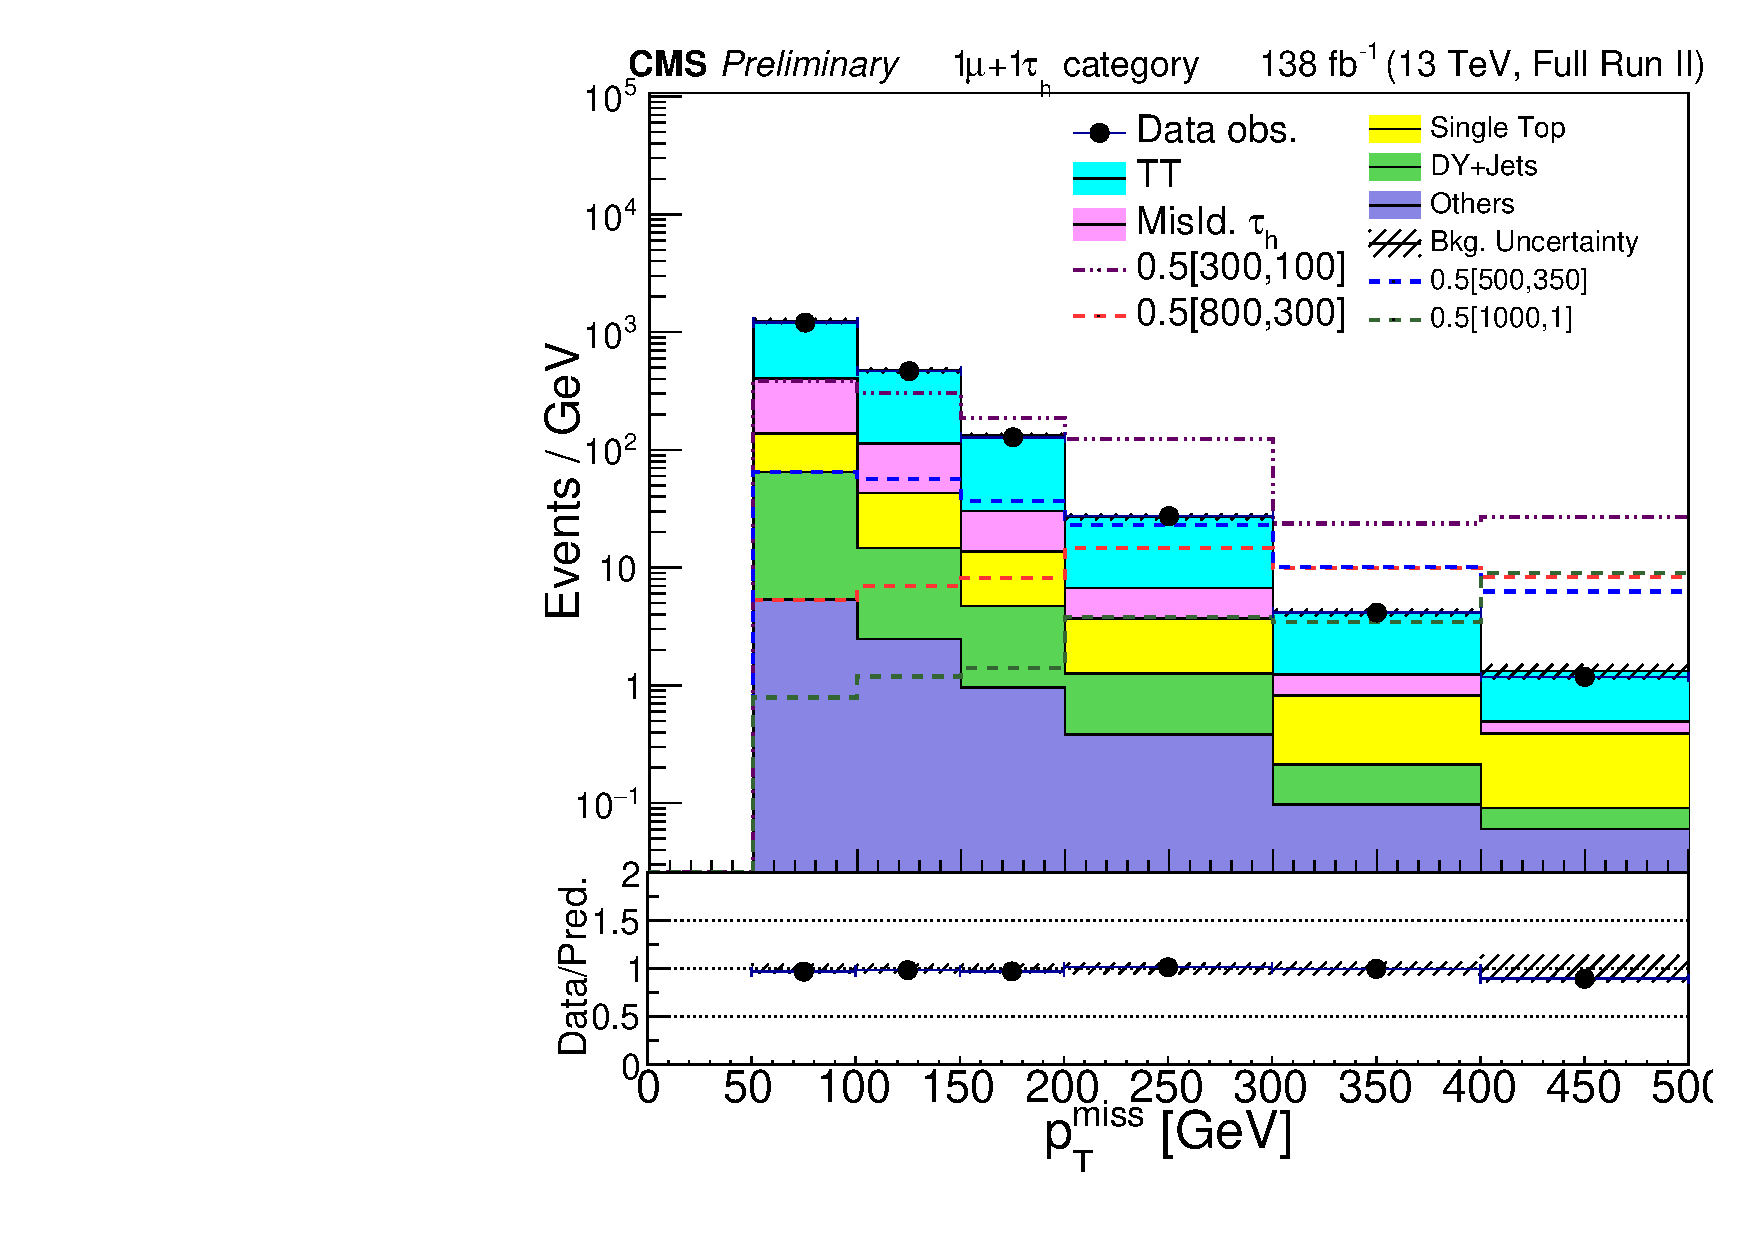
\includegraphics[width=0.32\textwidth]{Fig/Met_1Mu1Tau_FullRun2.pdf}
	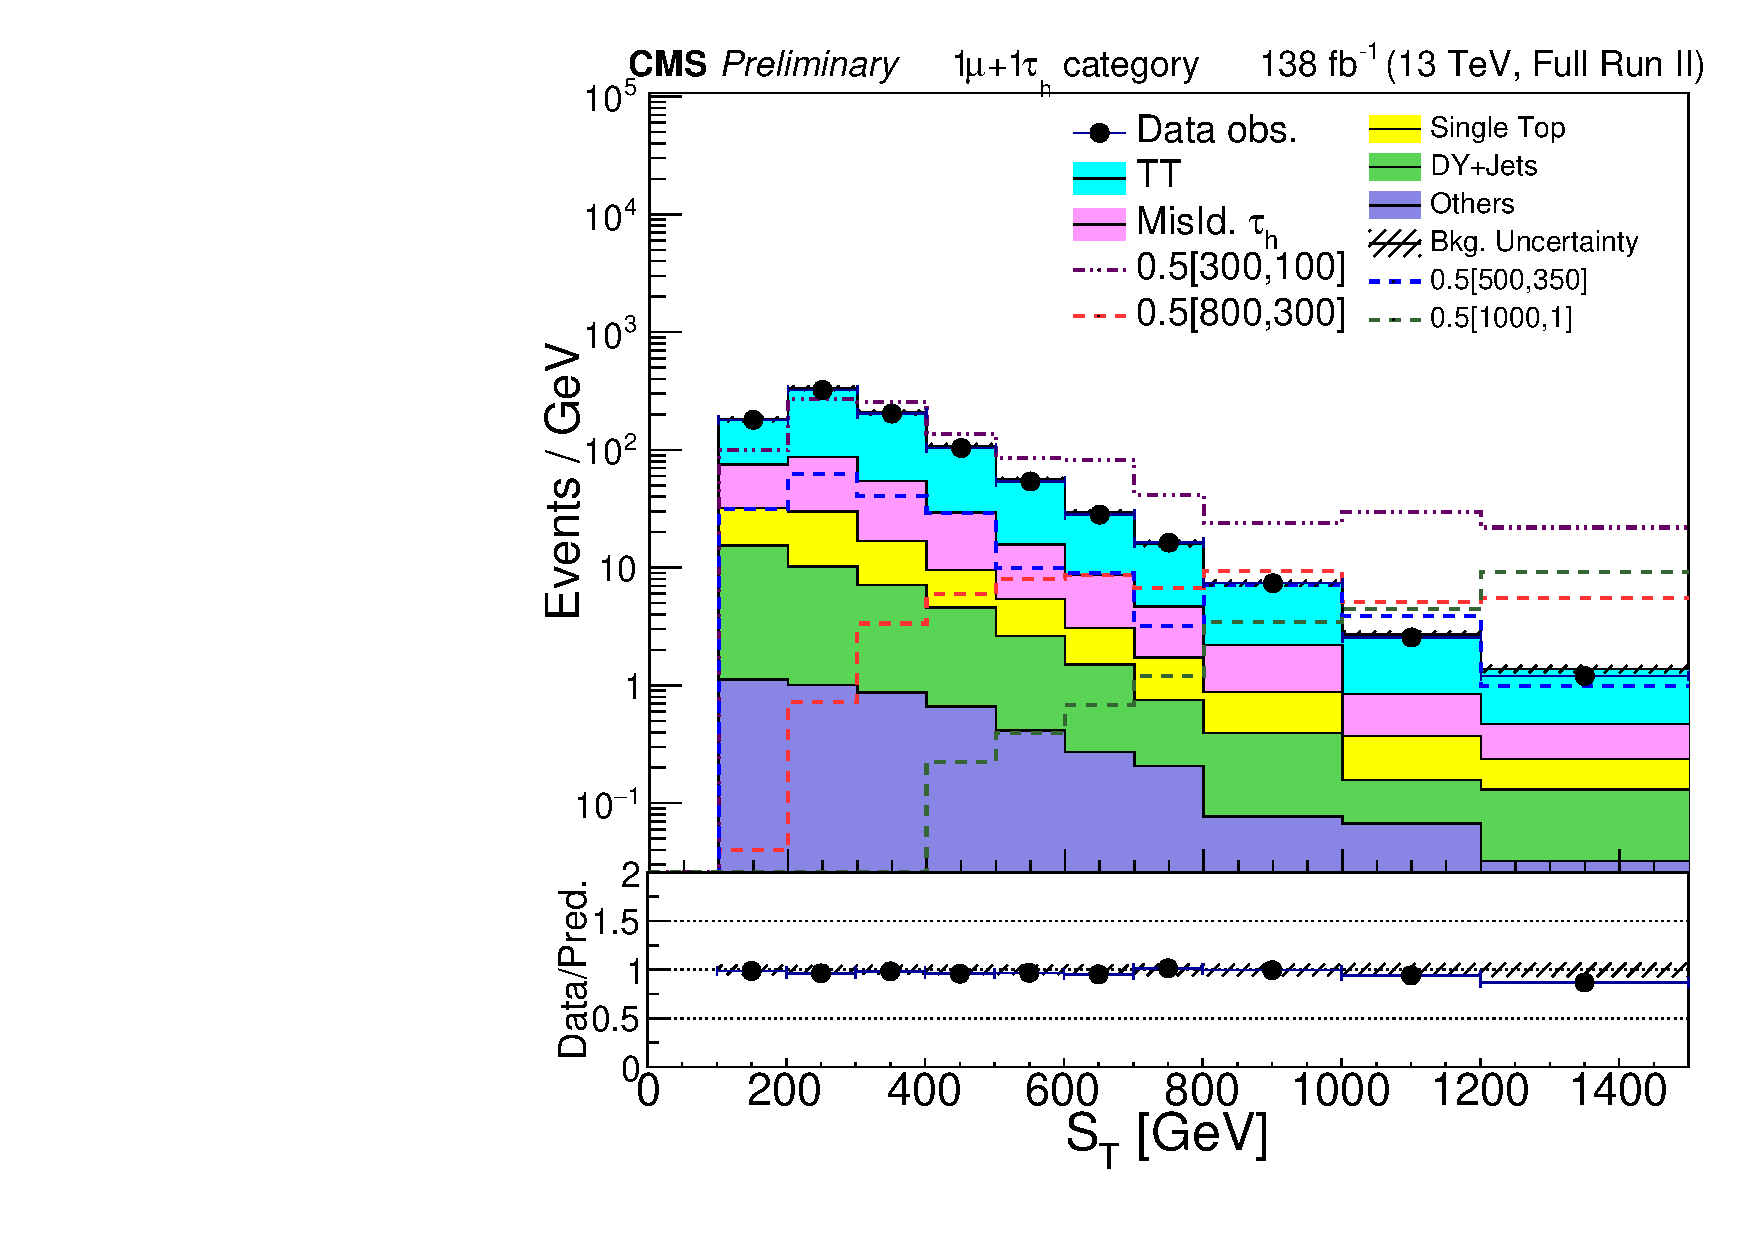
\includegraphics[width=0.32\textwidth]{Fig/Ht_1Mu1Tau_FullRun2.pdf}
	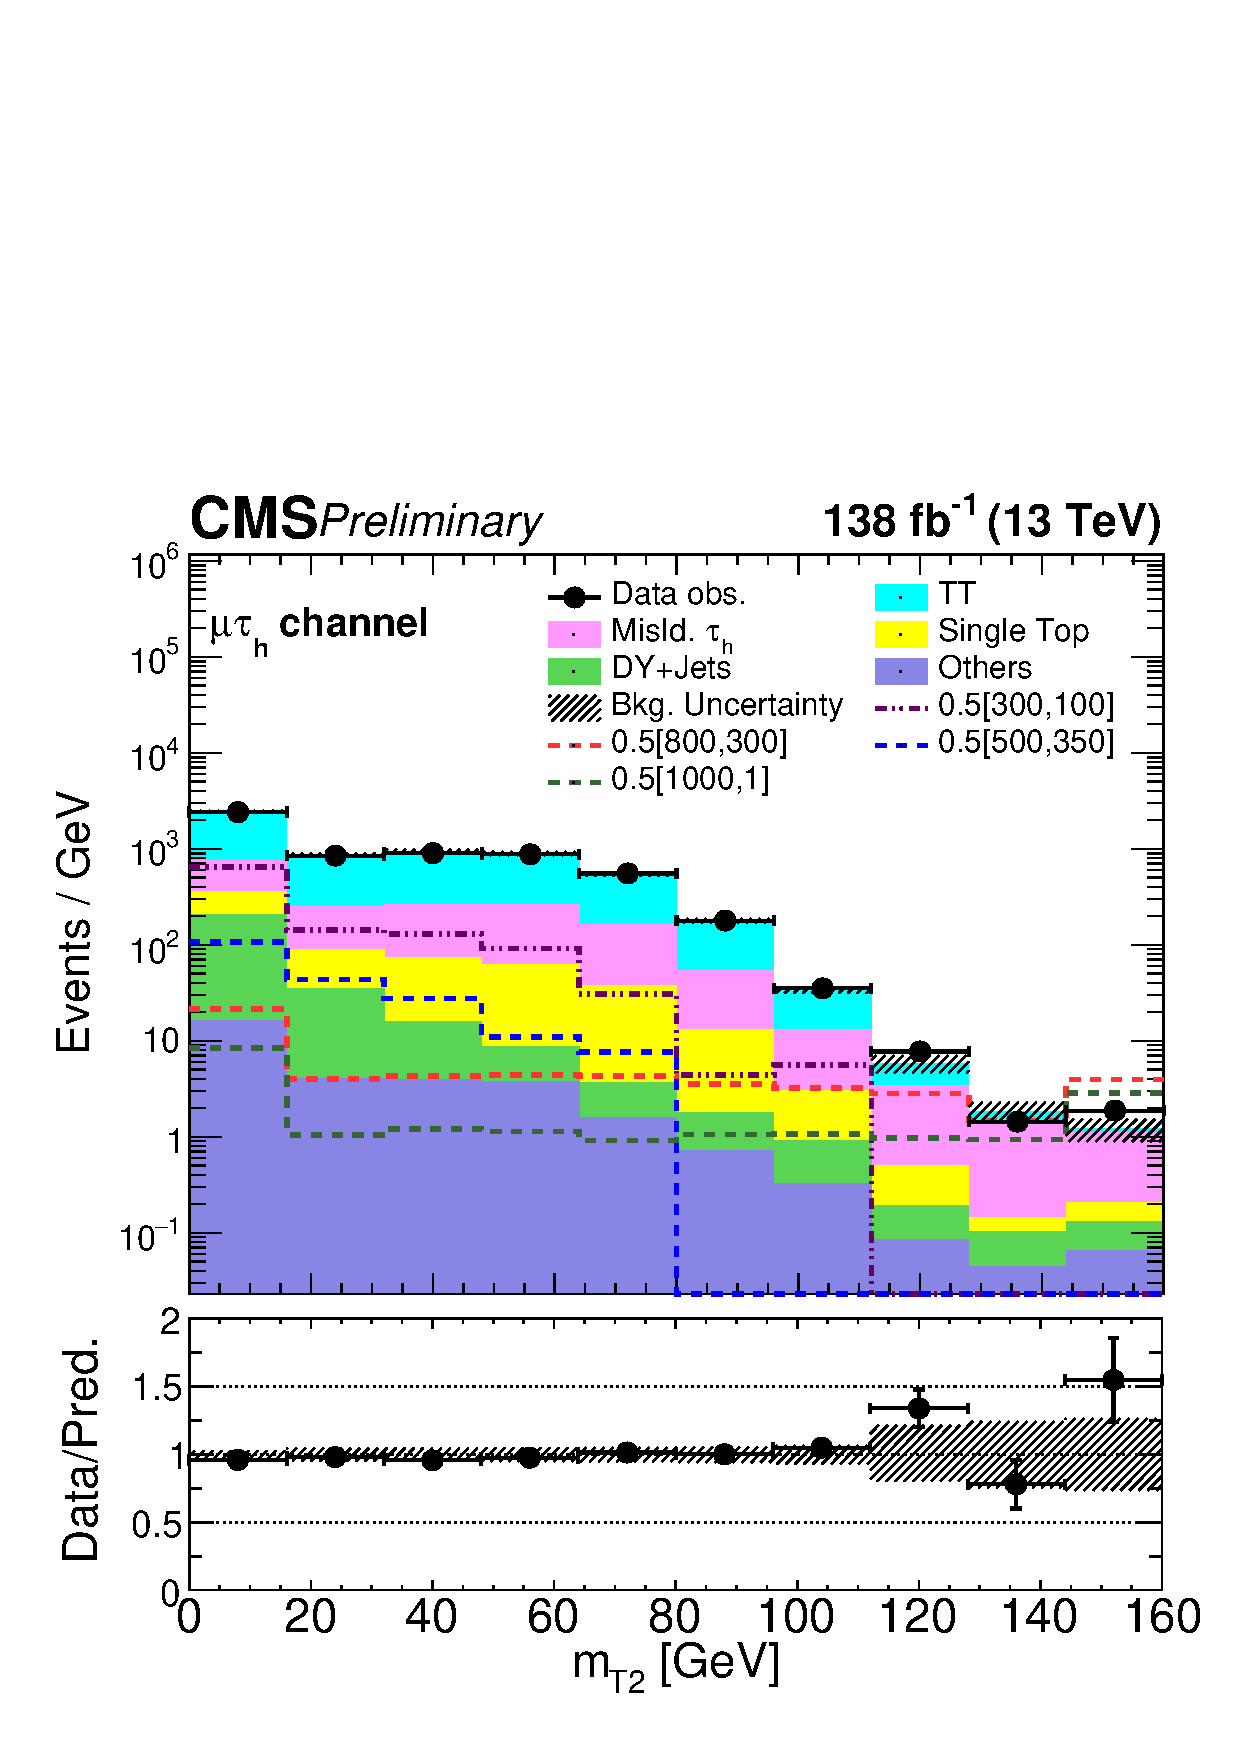
\includegraphics[width=0.32\textwidth]{Fig/Mt2_1Mu1Tau_FullRun2.pdf}
	\caption{
		Distributions of the search variables \ptmiss, \mTii,
		and \ST after event selection, for data and the predicted background, corresponding to the $\Pe\tauh$ category(upper row) and $\PGm\tauh$ category(lower row).
		The are presented for a few representative points corresponding to $ x = 0.5 $ and [$ m_{\PSQtDo} $, $ m_{\PSGczDo} $] = [300, 100], [500, 350], [800, 300], and [1000, 1]\GeV are overlaid.
		The lower panel of each plot indicates the ratio of the observed data to the background prediction.
		The shaded bands indicate the statistical and systematic uncertainties on the background, added in quadrature. The overflow events are included in the last bin.
	}
	\label{fig:data_mc_comp}
\end{figure}

\subsection{Background estimation}
In the sensitive bins the largest (prompt) contribution is from $\ttbar$ and $\PQt\PW$, which are expected because of its large cross section and it's event topology, which is very similar to our signal. For $\ttbar$ and $\PQt\PW$ scale-factors are derived in a data driven way from a $\ttbar$ and $\PQt\PW$ enriched control region to correct for the background modelling uncertainty. Details are discussed in Section \ref{ttbar_SF}.\\
The other major background contribution in the sensitive bins is from fakes (mostly from hadronic and semi-leptonic $\ttbar$ events). We predict the fake background using a data-driven method discussed in Section \ref{fakeBkg_est}.\\
The Drell-Yan background is estimated from MC simulation with \PZ-$\pt$ re-weighting applied. The other small backgrounds are estimated from MC, with the recommended corrections/ scale-factors (SF) applied.

\subsubsection{Tau lepton pairs from top production}\label{ttbar_SF}
The estimation of the background from \ttbar and single top ($\PQt\PW$) events in which there are two genuine \tauh decays (or one genuine \tauh decay and a genuine lepton) is based on the method described in Refs.~\cite{CMS:2019lrh, Sirunyan:2645851}. The predicted yields in each signal region (SR) bin from simulation are multiplied by correction factors derived in a control region (CR) enriched in \ttbar and single top events (collectively called a top-enriched CR). This CR is identified by selecting events with an oppositely charged $\Pe\PGm$ pair. The selection criteria are similar to that of SR selections with \tauh replaced by an electron or a muon. The overall purity of $\ttbar+\PQt\PW$ events is $\geq90\%$. For a given SR region $(i\text{-th bin})$ we define the scale factor as:\\
\begin{equation}
	SF_{i}=\frac{N_{\text{CR},i}^{\text{data}}}{N_{\text{CR},i}^{\text{all~MC}}}
	\label{eqn:sf}
\end{equation}
where the numerator is the number of events selected in data and the denominator is the total expected events in the $i$th CR. The corrected \ttbar yield in simulation in each bin of the SR is then obtained as:
\begin{equation}
SR_{i}^{\text{corr}~\ttbar}=SR_{i}^{\ttbar~\text{MC}}\times SF_{i} = SR_{i}^{\ttbar~\text{MC}}\times\frac{N_{\text{CR},i}^{\text{data}}}{N_{\text{CR},i}^{\text{all~MC}}}
\end{equation}
The SFs are about 10\% in the most of the bins.

\subsubsection{Misidentified hadronically decaying tau lepton candidates}\label{fakeBkg_est}
In the $\Pe\tauh$ and $\PGm\tauh$ categories, a major background contribution arises from semileptonic single top and \ttbar events where there is a genuine electron or muon, and a jet is misidentified as $\tauh$.
This background is estimated by selecting a side band region (SbR) where all the signal region selections are applied, except that the $\tauh$ candidate is required to pass the very loose (VL) WP but fail the tight (T) identification criteria; this identification requirement is indicated as ``VL \&\& !T'' in the following discussion.
The yields from this side band region are extrapolated to obtain the contribution from misidentified \tauh candidates to the $\ell\tauh$ signal region.
The extrapolation factor is determined in a CR~\cite{CMS:2019eln} enriched in {\PW}+jets events containing a misidentified \tauh candidate.
This CR is extracted from data by requiring exactly one \PGm and exactly one $\tauh$, $\ptmiss\ge50$ \GeV and $60<\mT<130$ \GeV, where \mT is the transverse mass computed using \ptvecmiss and the muon momentum.
Events with any \PQb-tagged jet passing the loose WP are vetoed to make this CR orthogonal to the signal region.
The fraction of {\PW}+jets events in this CR is calculated to be $\approx83\%$ from simulation.
The remaining contribution from non {\PW}+jets events is estimated from simulation and subtracted from the data.
%and non W+jets contributions are subtracted using Monte Carlo.
The extrapolation factor ($R$) is defined in this CR as,
%\begin{linenomath}
	\begin{equation}
	R =
	\frac{N_\text{data}^\text{CR} (\tauh^{\text{T}}) - N_\text{non-{\PW}+jets MC}^\text{CR} (\tauh^{\text{T}})}
	{N_\text{data}^\text{CR} (\tauh^{\text{VL \&\& !T}})-N_\text{non-{\PW}+jets MC}^{\text{CR}}(\tauh^{\text{VL \&\& !T}})} .
	\label{eq:transferFactor}
	\end{equation}
%\end{linenomath}
Here $N_{\text{data}}^{\text{CR}}$ is the number of events in the {\PW}+jets CR obtained from data, and $N_\text{MC, non-{\PW}+jets}^\text{CR}$ is the number of simulated events (except {\PW}+jets) in the same CR.
It is evident that $R$ facilitates the transfer from a region with misidentified \tauh candidates satisfying the ``VL \&\& !T'' requirement ($\tauh^{\text{VL \&\& !T}}$) to that with misidentified \tauh candidates satisfying the ``T" requirement ($\tauh^{\text{VL \&\& !T}}$).
The value of $R$ is calculated as a function of the \pt and $\eta$ of the \tauh candidate and is found to vary between 15-30\% with \pt and $\eta$.
It is found using simulated {\PW}+jets events that $R$ varies by ${\approx}15\%$ percent depending on the flavour of the parton corresponding to the jet that is misidentified as a \tauh. Since the jet flavor cannot be reliably determined in data, an uncertainty of 15\% in $R$ is included.
%The background coming from the misidentification of jets as $\tauh$ is determined in the SR from sideband as:
The contribution from misidentified \tauh candidates to the $\ell\tauh$ signal region is then evaluated as,
%\begin{linenomath}
	\begin{equation}
	N^{\text{misid, SR}} = R N^{\text{misid, SbR}} = R \left[N_{\text{data}}^{\text{SbR}} - N_{\text{MC, genuine \tauh}}^{\text{SbR}}\right],
	\end{equation}
%\end{linenomath}
where $N_{\text{data}}^{\text{SbR}}$ is the number of events obtained in the side band region from data, and $N_{\text{MC, genuine \tauh}}^{\text{SbR}}$ represents the contribution to the side band region from simulated events where the $\tauh$ candidate is genuine.
Thus, the number of side band events with a misidentified \tauh candidate ($N^{\text{misid, SbR}}$) is obtained by subtracting $N_{\text{MC, genuine \tauh}}^{\text{SbR}}$ from $N_{\text{data}}^{\text{SbR}}$.
Finally, $N^{\text{misid, SbR}}$ is multiplied by $R$ which extrapolates the yields from the side band (where the \tauh candidate passes the ``VL \&\& !T'' requirement) to the signal (where the \tauh candidate passes the ``T'' requirement) region.

\subsection{Systematics}
Several systematic uncertainties are taken into account for the prediction of the final signal and backgrounds yields. Among them the most prominent ones are uncertainty due to identification and isolation of \tauh (3.5\%) and that associated with \ttbar SFs (4.0\%). Apart from these two, other uncertainties that are considered are due to jet energy scales (JES), jet energy resolution (JER), \PQb-tagging, the effect of unclustered components in calculating \ptmiss, parton flavor dependence of the fake rates, trigger and \tauh energy scale. In addition, theoretical uncertainties are obtained by varying the factorization and renormalization scales.
$\textsc{FastSim}\to\textsc{Geant4}$ corrections (for signal only) are also included. JER uncertainty, uncertainty coming from the flavor dependence of the fake rates and the uncertainty from the $\textsc{FastSim}$ \ptmiss resolution are assumed to be correlated across the three years. Other uncertainties are taken to be uncorrelated across the different years but assumed correlated across different SR bins. The statistical uncertainties are also take into account and considered to be uncorrelated across different SR bins. The tabulated sources of systematic uncertainties are modelled by log-normal distributions~\cite{CMS-NOTE-2011-005} in the likelihood function used for the statistical interpretation of the results. The range of relative uncertainties for the $\PGm$$\tauh$ category for full Run 2 is shown in Table \ref{tab:syst_range}. A similar impact is also expected for $\Pe$$\tauh$ category.
%\begin{center}
\begin{table}[htb!]
	\centering
	\small\addtolength{\tabcolsep}{-0.0pt}
	\caption{Range of relative uncertainties in $\PGm$$\tauh$ category from different sources on signal and background yields in full Run2.}
	\resizebox{\textwidth}{!}{
\begin{tabular}{|l|c|c|c|c|c|c|c|}\hline
	~Uncertainty source & $\ttbar$ & Fake & Single Top & Others & x = 0.5 & x = 0.5\\
	~  & ~ & ~ & ~ & ~ & [1000,1] & [800,300]\\
	\hline
	Signal cross-section & -&-&-&-&-& $\pm 9.5$\%\\
	FastSim \ptmiss resolution &
	-&
	-&
	-&
	-&
	0.0-0.2\%&
	0.1-9.8\%\\
	
	\tauh FastSim/FullSim &
	-&
	-&
	-&
	-&
	0.0-0.2\%&
	0.1-9.8\%\\
	
	$\PGm$ FastSim/FullSim &
	-&
	-&
	-&
	-&
	0.4-1.4\%&
	0.7-1.0\%\\
	
	JER &
	-&
	0.1-4.4\%&              
	0.2-35.4\%&
	0.0-38.0\% &      
	0-11.9\%&   
	0.4-4.7\%\\
	
	JEC &
	-&                 
	0.1-9.0\%&
	0.0-35.8\%&                
	0.1-151.1\%&       
	0-13.5\%&   
	0.0-19.2\%\\
	
	QCD scale &
	-  &               
	3.3-56.0\%&
	3.1-16.2\% &                    
	0.9-20.4\%&          
	0.1-3.2\%&     
	0.0-2.1\%\\
	
	\tauh Id-iso &
	3.06-4.04\%&
	0.48-7.0\%&              
	3.08-4.1\% &                                  
	2.9-4.1\%&                 
	2.30-4.2\%&    
	2.9-4.3\%\\
	
	Pileup &
	 -  &               
	 0.0-1.6\%&
	 0.26-2.6\%&                                    
	 0.0-4.4\%&                 
	 0.1-8.8\%&     
	 0.0-0.9\%\\
	 
	 \ptmiss Unclustered energy &
	 -     &            
	 0.0-3.2\%&
	 0.0-25.4\%&                                    
	 0.1-25.5\%&                
	 0-72.186\%&    
	 0-7.1\%\\
	 
	 b-tagging &
	 -     &            
	 0.2-2.5\%&
	 0.0-2.4\%&                                     
	 1.5-10.9\%&                
	 0.1-0.5\%&     
	 0.0-0.4\%\\
	 
	 \tauh energy scale &
	 0.0-4.6\% &
	 0.0-1.7\% &              
	 0-4.6\% &                                     
	 0.0-7.2\% &                
	 0-3.2\% &      
	 0-8.9\%\\
	 
	 $\ttbar$ SF &
	 3.4-30.4\%&             
	 0-0\%&  
	 3.4-37.0\%&                                        
	 0-0\%&                     
	 0-0\%&         
	 0-0\%\\
	 
	 \tauh fake rate &&&&&&\\
	 (parton flavour) &
	  - &
	  $\pm$ 15\% &
	  - &
	  - &  
	  - & 
	  -\\
	  \hline
\end{tabular}}
	\label{tab:syst_range}
\end{table}
%\end{center}

\subsection{Results}
\begin{table}
\centering
\caption{Event yields along with statistical and systematic uncertainties in the 2016, 2017 and 2018 analyses combined, for the $\Pe\tauh$ category for different background sources and the total background and number of events observed in data in the 15 search bins.}
	\small\addtolength{\tabcolsep}{-4pt}
	\begin{tabular}{l c c c c c c}
\hline
%\\[\cmsTabSkipSmall]
SR& 
$\ttbar$ & 
Single top & 
DY $+$ Other SM &
Misid. \tauh &  
Total bkg. & 
Data\\%[\cmsTabSkip]
\hline
\rule{0pt}{2.75ex}
1 & 
$11574^{+50+634}_{-50-651}$ & 
$1210^{+15+62}_{-15-66}$ & 
$793^{+34+74}_{-34-90}$ &  
$2646^{+29+500}_{-29-498}$ &
$16222^{+69+658}_{-68-675}$ & 
$15744$\\
\rule{0pt}{2.75ex}
2 & 
$12239^{+50+568}_{-50-630}$ & 
$799^{+12+50}_{-12-50}$ & 
$717^{+26+45}_{-26-55}$ &  
$2619^{+30+504}_{-30-503}$ &
$16374^{+65+598}_{-65-658}$ & 
$15605$\\
\rule{0pt}{2.75ex}

3 & 
$1151^{+15+57}_{-15-63}$ & 
$90^{+4+11}_{-4-9}$ & 
$84^{+7+8}_{-7-6}$ &
$277^{+10+56}_{-10-61}$ &  
$1601^{+20+64}_{-20-73}$ & 
$1524$\\
\rule{0pt}{2.75ex}

4 & 
$779^{+13+43}_{-13-46}$ & 
$123^{+5+10}_{-5-9}$ & 
$55^{+6+4}_{-6-8}$ &
$92^{+6+20}_{-6-21}$ &  
$1048^{+16+46}_{-16-49}$ & 
$1039$\\
\rule{0pt}{2.75ex}

5 & 
$381^{+8+34}_{-8-35}$ & 
$65^{+4+9}_{-4-7}$ & 
$30^{+5+4}_{-5-3}$ &  
$39^{+5+14}_{-5-20}$ &
$514^{+11+38}_{-11-41}$ & 
$520$\\
\rule{0pt}{2.75ex}

6 & 
$6984^{+40+335}_{-40-368}$ & 
$774^{+12+38}_{-12-43}$ & 
$78^{+11+35}_{-11-8}$ &  
$1989^{+24+370}_{-24-370}$ &
$9825^{+49+350}_{-49-382}$ & 
$9372$\\
\rule{0pt}{2.75ex}

7 & 
$4822^{+32+251}_{-32-285}$ & 
$290^{+7+18}_{-7-19}$ & 
$52^{+6+19}_{-6-6}$ &  
$1395^{+21+263}_{-21-263}$ &
$6559^{+39+263}_{-39-296}$ & 
$6222$\\
\rule{0pt}{2.75ex}

8 & 
$287^{+8+23}_{-8-24}$ & 
$18^{+2+2}_{-2-2}$ & 
$9.2^{+1.9+6.5}_{-1.9-1.1}$ &  
$104^{+6+20}_{-6-21}$ &
$418^{+10+24}_{-10-26}$ & 
$435$\\
\rule{0pt}{2.75ex}

9 & 
$251^{+7+17}_{-7-18}$ &  
$27^{+2+2}_{-2-2}$ & 
$3.2^{+1.3+2.8}_{-1.3-0.6}$ & 
$62^{+4+11}_{-4-11}$ &
$343^{+9+18}_{-9-18}$ & 
$303$\\
\rule{0pt}{2.75ex}

10 & 
$70^{+4+8}_{-4-9}$ & 
$12^{+1+1}_{-1-1}$ & 
$1.1^{+0.3+0.3}_{-0.3-0.3}$ & 
$17^{+2.6+3.7}_{-2.6-4.3}$ & 
$99^{+4.8+8.9}_{-4.8-9.4}$ & 
$95$\\
\rule{0pt}{2.75ex}

11 & 
$800^{+14+41}_{-14-44}$ & 
$87^{+4+5}_{-4-6}$ & 
$5.9^{+2.1+1.2}_{-2.1-2.0}$ &  
$257^{+8+48}_{-8-49}$ &
$1150^{+17+43}_{-17-47}$ & 
$1131$\\
\rule{0pt}{2.75ex}

12 & 
$575^{+11+35}_{-11-43}$ & 
$37^{+3+3}_{-3-3}$ & 
$6.4^{+2.1+8.1}_{-2.1-0.8}$ &  
$254^{+8+47}_{-8-48}$ &
$873^{+14+37}_{-14-46}$ & 
$921$\\
\rule{0pt}{2.75ex}

13 & 
$44^{+3+6}_{-3-6}$ & 
$5.7^{+1.1+1.0}_{-1.1-0.7}$ & 
$6.8^{+2.8+0.9}_{-2.8-3.3}$ & 
$40^{+3+7}_{-3-7}$ & 
$97^{+5+6}_{-5-7}$ & 
$114$\\
\rule{0pt}{2.75ex}

14 & 
$24^{+2+4}_{-2-4}$ & 
$2.6^{+0.7+0.3}_{-0.7-0.3}$ & 
$2.7^{+1.2+0.6}_{-1.2-0.9}$ & 
$13^{+2+2}_{-2-3}$ & 
$42^{+3+4}_{-3-4}$ & 
$49$\\
\rule{0pt}{2.75ex}

15 & 
$5.8^{+0.9+1.8}_{-0.9-1.7}$ & 
$1.5^{+0.6+0.2}_{-0.6-0.2}$ & 
$0.3^{+0.1+0.1}_{-0.1-0.1}$ & 
$9.5^{+1.6+2.3}_{-1.6-2.2}$ & 
$17^{+2+3}_{-2-2}$ & 
$17$\\
\rule{0pt}{2.75ex}

Total & 
$39985^{+92+2006}_{-92-2176}$ &  
$3543^{+26+211}_{-26-217}$ & 
$1844^{+46+171}_{-46-170}$ & 
$9811^{+56+1858}_{-56-1861}$ &
$55183^{+120+2747}_{-120-2876}$ & 
$53122$\\
\hline
\end{tabular}

	\label{tab:EleTau_fullRun2}
\end{table}

\begin{table}
	\centering
	\caption{Event yields along with statistical and systematic uncertainties in the 2016, 2017 and 2018 analyses combined, for the $\PGm\tauh$ category for different background sources and the total background and number of events observed in data in the 15 search bins.}
	\small\addtolength{\tabcolsep}{-4pt}
	\begin{tabular}{l c c c c c c }
\hline
%\\[\cmsTabSkipSmall]
SR& 
$\ttbar$ & 
Single top & 
DY + Other SM &   
Misid. \tauh &
Total bkg. &
Data\\%[\cmsTabSkip]
\hline
\rule{0pt}{2.75ex}
1 & 
$20947^{+70+1147}_{-70-1178}$ & 
$2152^{+21+109}_{-21-118}$ & 
$2340^{+61+338}_{-61-299}$ &  
$5391^{+41+1010}_{-41-1007}$ &
$30801^{+104+1232}_{-104-1267}$ & 
$29475$\\
\rule{0pt}{2.75ex}

2 & 
$18973^{+65+876}_{-65-972}$ & 
$1206^{+16+75}_{-16-76}$ & 
$1359^{+37+92}_{-37-97}$ & 
$4340^{+38+827}_{-38-828}$ &
$25861^{+85+942}_{-85-1017}$ & 
$25055$\\
\rule{0pt}{2.75ex}

3 & 
$1624^{+18+80}_{-18-90}$ & 
$126^{+5+14}_{-5-12}$ & 
$151^{+10+14}_{-10-14}$ & 
$424^{+12+86}_{-12-92}$ & 
$2323^{+25+97}_{-25-106}$ & 
$2273$\\
\rule{0pt}{2.75ex}

4 & 
$1258^{+17+70}_{-17-75}$ & 
$ 182^{+6+14}_{-6-13}$ & 
$98^{+11+8}_{-11-27}$ &  
$163^{+8+36}_{-8-37}$ &
$1700^{+23+75}_{-23-99}$ & 
$1678$\\
\rule{0pt}{2.75ex}

5 & 
$579^{+10+52}_{-10-54}$  & 
$95^{+4+13}_{-4-10}$ & 
$45^{+6+4}_{-6-5}$ &  
$47^{+6+20}_{-6-28}$ &
$764^{+14+58}_{-14-62}$ & 
$800$\\
\rule{0pt}{2.75ex}

6 & 
$13094^{+56+633}_{-56-692}$  & 
$1358^{+17+68}_{-17-75} $ & 
$193^{+13+55}_{-13-28}$ &  
$4132^{+34+765}_{-34-765}$ &
$18752^{+69+663}_{-69-723}$ & 
$18412$\\
\rule{0pt}{2.75ex}

7 & 
$7754^{+42+409}_{-42-459}$ & 
$453^{+10+30}_{-10-32}$ & 
$85^{+8+29}_{-8-7}$ &  
$2398^{+27+449}_{-27-450}$ &
$10685^{+51+438}_{-51-477}$ & 
$10441$\\
\rule{0pt}{2.75ex}

8 & 
$444^{+10+36}_{-10-37}$ & 
$33.4^{+3+4}_{-3-3.2}$ & 
$17^{+3+8}_{-3-1.8}$ &  
$172^{+7+33}_{-7-34}$ &
$666^{+13+40}_{-13-41}$ & 
$638$\\
\rule{0pt}{2.75ex}

9 & 
$414^{+10+29}_{-10-31}$ &  
$44.5^{+3.0+3.5}_{-3.0-3.5}$ & 
$7.0^{+3.0+1.5}_{-3.0-2.4}$ & 
$88^{+6+17}_{-6-18}$ &
$554^{+12+30}_{-12-33}$ & 
$565$\\
\rule{0pt}{2.75ex}

10 & 
$107^{+5+13}_{-5-13}$ & 
$16^{+2+2}_{-2-2}$ & 
$1.9^{+1.0+2.9}_{-1.0-0.5}$ &  
$24^{+3+6}_{-3-6}$ &
$149^{+6+14}_{-6-14}$ & 
$132$\\
\rule{0pt}{2.75ex}

11 & 
$1332^{+18+67}_{-18-78}$ &
$153^{+6+9}_{-6-10}$ & 
$12^{+4+6}_{-4-1}$ &  
$435^{+11.1+81}_{-11-83}$ &
$1931^{+22+72}_{-22-85}$ & 
$2027$\\
\rule{0pt}{2.75ex}

12 & 
$905^{+15+56}_{-15-62}$ & 
$59^{+4+4}_{-4-5}$ & 
$29^{+5+8}_{-5-3}$ &  
$391^{+10+72}_{-10-74}$ &
$1383^{+19+62}_{-19-66}$ & 
$1333$\\
\rule{0pt}{2.75ex}

13 & 
$70^{+4+9}_{-4-9}$ &
$46^{+4+8}_{-4-8}$ & 
$5.9^{+1.1+0.6}_{-1.1-0.6}$ & 
$6.7^{+2.0+0.6}_{-2.0-3.0}$ &  
$128^{+6+10}_{-6-10}$ & 
$111$\\
\rule{0pt}{2.75ex}

14 & 
$39^{+3+6}_{-3-6}$ &
$3.1^{+0.9+0.2}_{-0.9-0.2}$ & 
$2.3^{+0.7+0.2}_{-0.7-0.3}$ &  
$25^{+3+5}_{-3-6}$ &
$70^{+4+7}_{-4-7}$ & 
$69$\\
\rule{0pt}{2.75ex}

15 & 
$8.1^{+1.2+2.5}_{-1.2-2.5}$ & 
$2.7^{+0.8+0.4}_{-0.8-0.3}$ & 
$0.8^{+0.2+0.2}_{-0.2-0.2}$ & 
$8.3^{+1.5+1.5}_{-1.5-1.5}$ & 
$20^{+2+3}_{-2-3}$ & 
$18$\\
\rule{0pt}{2.75ex}

Total & 
$67548^{+125+3395}_{-125-3676}$ &  
$5890^{+35+350}_{-35-360}$ & 
$4348^{+75+510}_{-75-449}$ & 
$18083^{+75+3398}_{-75-3405}$ &
$95870^{+167+4843}_{-167-5044}$ & 
$93072$\\
\hline
\end{tabular}

	\label{tab:MuTau_fullRun2}
\end{table}
The observed and expected yields (along with their uncertainties) are presented in all 15 search bins, in Tables \ref{tab:EleTau_fullRun2} and \ref{tab:MuTau_fullRun2} for the $\Pe\tauh$ and $\PGm\tauh$ respectively.
The test statistic used for the interpretation of the result is the profile likelihood ratio $ q_{\mu} = -2 \ln{(\mathcal{L}_{\mu} / \mathcal{L}_{\text{max}})} $, where $ \mathcal{L}_{\mu} $ is the maximum likelihood for a fixed signal strength $ \mu $, and $ \mathcal{L}_{\text{max}} $ is the global maximum of the likelihood~\cite{CMS-NOTE-2011-005}. We set upper limits on signal production at 95\% confidence-level (\CL) using a modified frequentist approach and the \CLs criterion~\cite{JUNK1999435, Read_2002}, implemented through an asymptotic approximation of the test statistic \cite{Cowan2011}. In this calculation all the background and signal uncertainties are modelled as nuisance parameters and profiled in the maximum-likelihood fit. Final results are obtained by combining the yields from 2016, 2017 and 2018 data sets, in both $\Pe\tauh$ and $\PGm\tauh$ categories. The results are presented as observed and expected exclusion limits in the top squark and LSP mass plane in Figure~\ref{fig:2Dlimit}.
Top squark masses up to 1060 \GeV (850 \GeV) are excluded for a nearly massless LSP (LSP mass 360 \GeV). The limits become weaker with decreasing $ \Delta m = m_{\PSQtDo} - m_{\PSGczDo} $, corresponding to a parameter space with final-state particles having a lower momentum and hence less sensitivity.


\begin{figure}[htb!]
	\centering
	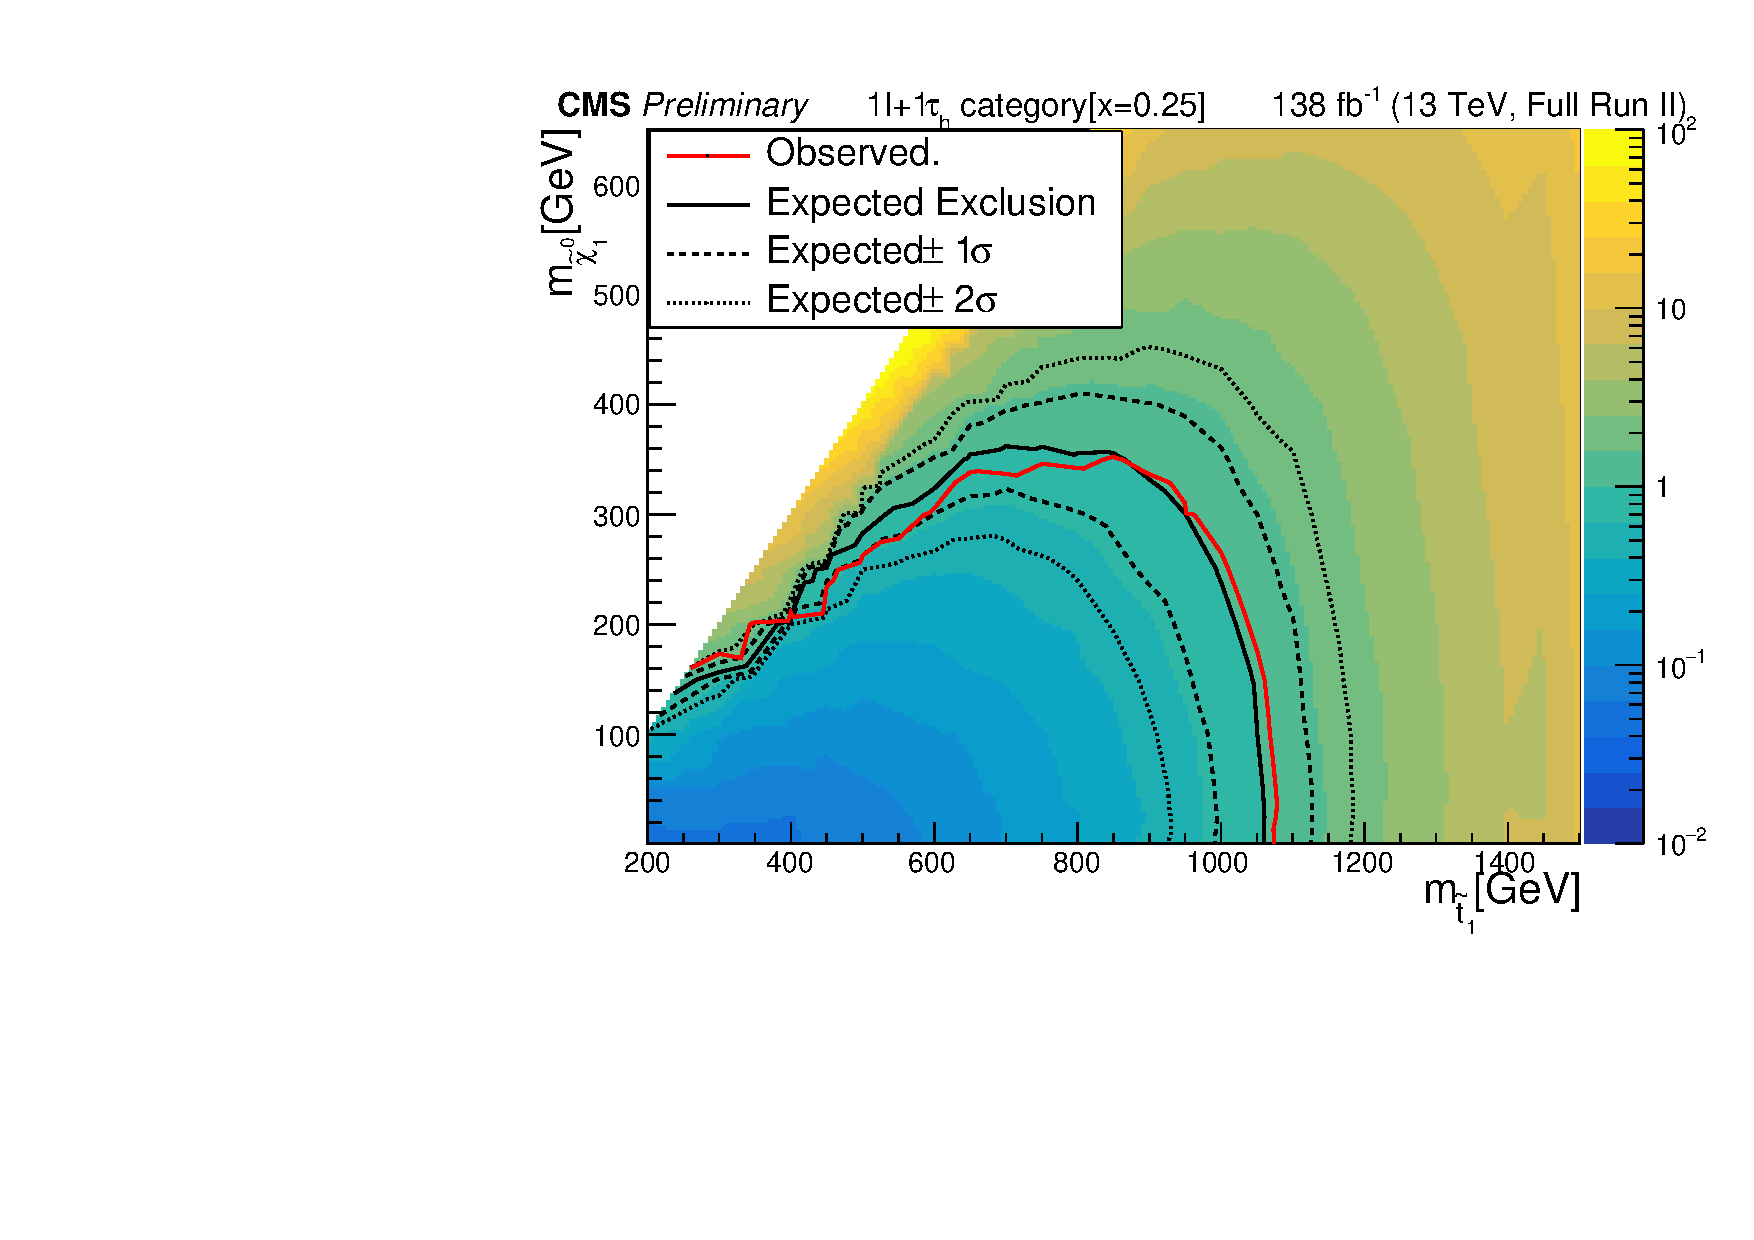
\includegraphics[width=0.4\textwidth]{Fig/exclusion0p25_LTau_FullRun2_Aug4.pdf}
	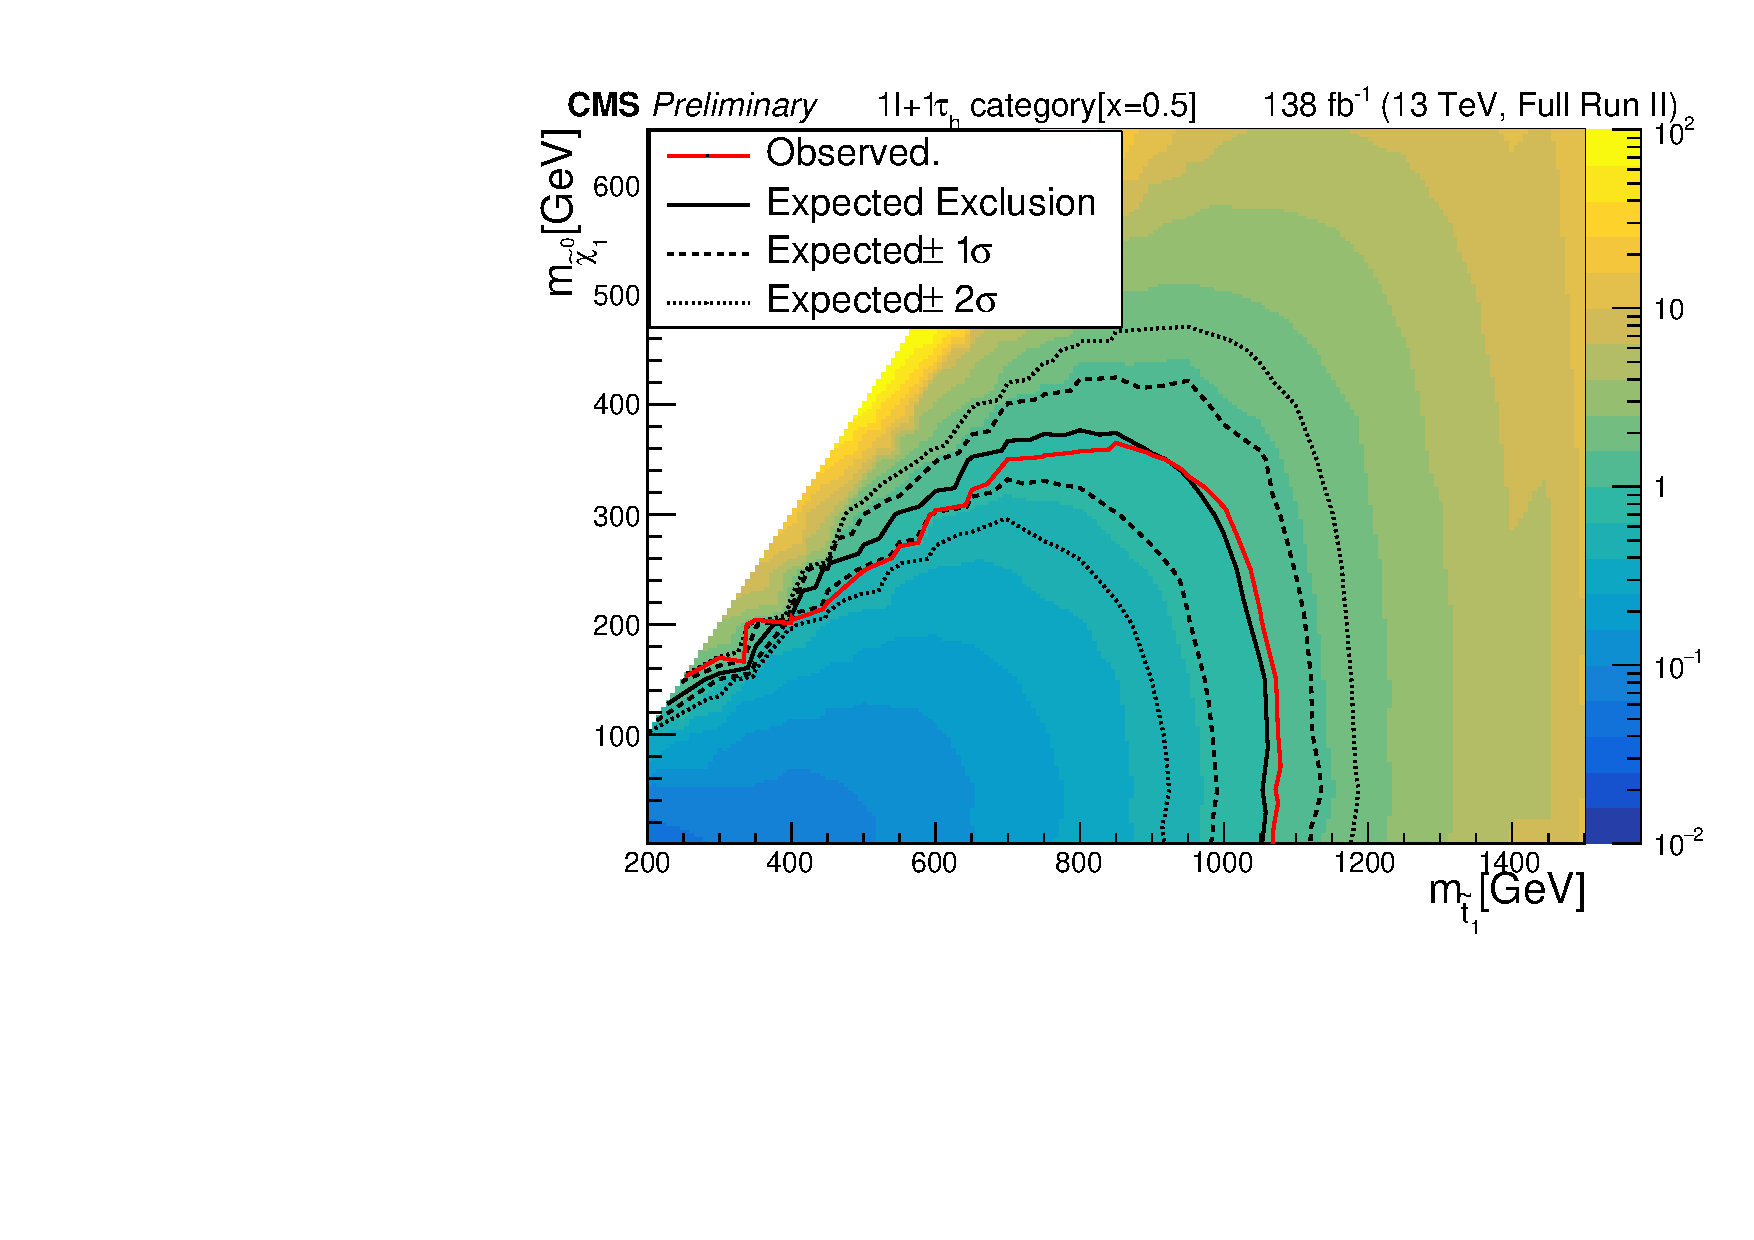
\includegraphics[width=0.4\textwidth]{Fig/exclusion0p5_LTau_FullRun2_Aug4.pdf}
	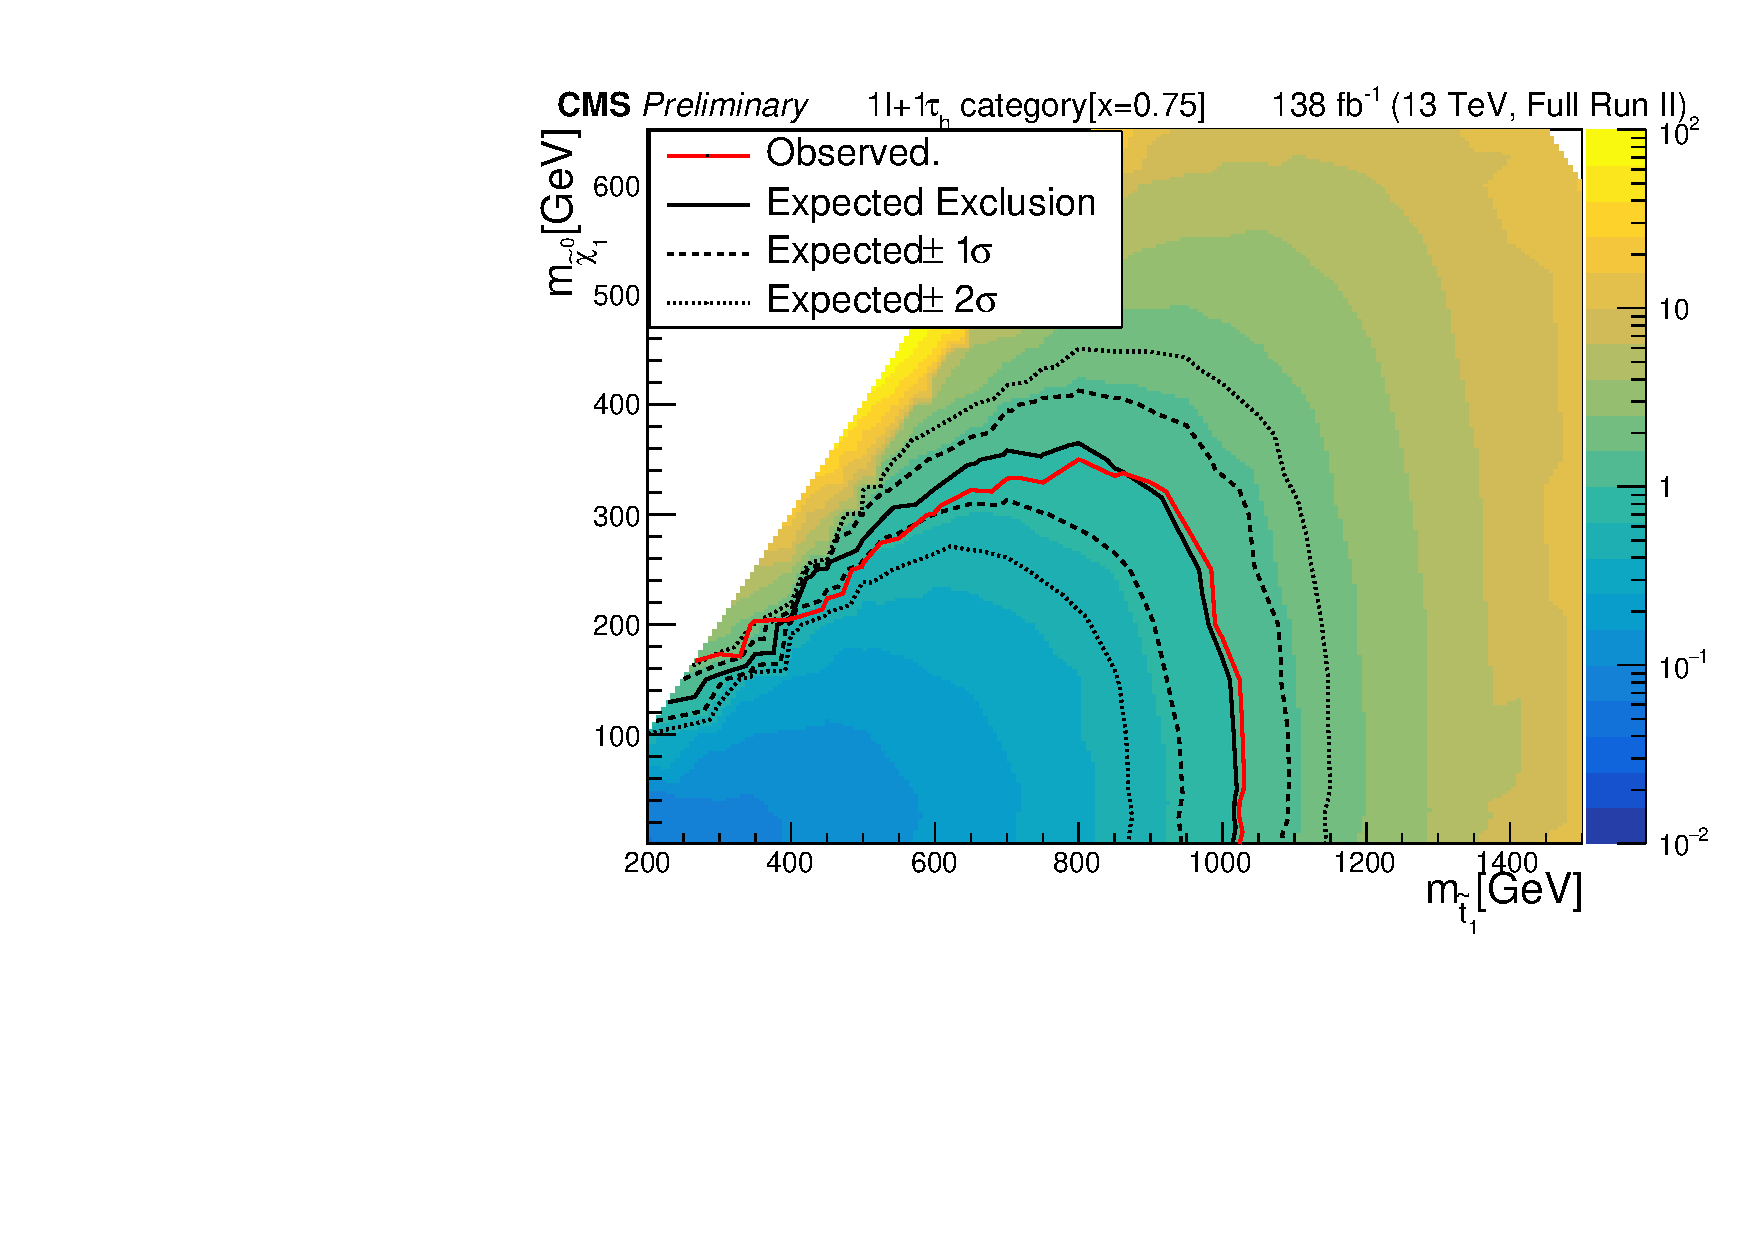
\includegraphics[width=0.4\textwidth]{Fig/exclusion0p75_LTau_FullRun2_Aug4.pdf}
	
	\caption{
		Exclusion limits at 95\% \CL for the pair production of top squarks decaying to $\ell\tauh$ ($\PGm\tauh+\Pe\tauh$) final states, displayed in the $ {m_{\PSQtDo}}$-$m_{\PSGczDo} $ plane for $x= 0.25$ (upper left), $0.5$ (upper right) and $0.75$ (lower) as described in Eq.~(\ref{eq:mass}). The color axis represents the observed limit in the cross section, while the black (red) curve represent the expected (observed) mass limits. The signal cross sections are evaluated using NNLO plus next-to-leading logarithmic (NLL) calculations. The solid curve represent the central values. The dashed red curves indicate the region containing 68\% of the distribution of limits expected under the background-only hypothesis. 
	}
	\label{fig:2Dlimit}
\end{figure}

\section{Summary}
In this report, two different analyses are presented. In the first analysis the measurement of the rate of Higgs boson production associated with \ttbar pair in a final state involving one \tauh and one electron or muon is presented. The signal strength is found to be consistent with SM prediction within the error bar. The second analysis is related to the search for top squark pair production in a final state that contains one \tauh and one electron or muon. Theoretically this result is motivated to
explore the higgsino-like and high $\tan\beta$ parameter space of SUSY models. No significance deviation is found from the SM prediction. Top squark mass up to 1060 \GeV is excluded for a nearly massless neutralino.
\clearpage
\bibliographystyle{utphys.bst}
\bibliography{synopsis.bib}
\end{document}